% \chapter{Observational Facilities}

% \section{Introduction}

% Until '900 astronomy was limited in the visual bands and human eye only detector:

% \begin{itemize}
%     \item $\lambda: 4000-7000$ Å
%     \item Resolution: \textasciitilde arcmin.
    
%     e.g. luna ~ 1 arcmin (resolvable), galaxy cluster ~ arcsec (not resolvable)
%     \item Field of view: \textasciitilde 160 deg (even too big)
%     \item Depth: \textasciitilde +6/+8 mag
% \end{itemize}

% Telescopes and detectors have revolutionized the fields in terms of:

% \begin{itemize}
%     \item Angular resolution
%     \item Depth
%     \item Surface brightness
%     \item Frequency range
% \end{itemize}

% \section{Telescopes and detectors}

% Several telescopes and detectors have been developed to extend the different fields of astronomy:

% \subsubsection{EHT - Angular resolution}
% The nearby supermassive black hole in the Messier 87 galaxy (2019) was detected by the Event Horizon Telescope (EHT) with a resolution of \textasciitilde 50 $\mu$arcsec.

% \subsubsection{HST - Depth}
% Hubble Space Telescope (HST) has an extreme deep field 22.5 days of exposure time →
% depth 31 mag!

% \subsubsection{Dragonfly - Surface brightness}

% A problem was to find objects with low contrast compared to the background. This was reached only recently with the Dragonfly telescope.

% Dragonfly is a telescope made up by a mosaic of (20) Canon telephoto lenses on two mounts. The lenses all point to the same target in the sky: adding together all the images from the mosaic of lenses makes Dragonfly the equivalent of a one-metre telescope.

% Dragonfly reached ~32 mag/arcsec !! Significantly below current limit of 29 for normal telescope.

% One of the main discovers of Dragonfly was the discovery of two galaxies (NGC-1052-DF2 and DF4) made apparentely devoid of Dark Matter.

% Opposite result was found for Dragonfly 44: a galaxy whose mass is almost entirely Dark Matter:

% Using the W. M. Keck Observatory and the Gemini North telescope a research team found a galaxy whose mass is almost entirely Dark Matter. Even though it is relatively nearby, astronomers had missed the galaxy, named Dragonfly 44, for decades because it is very dim. It was discovered just recently when the Dragonfly Telephoto Array observed a region of the sky in the constellation Coma.

% \subsection{Frequency bands}

% %TODO: small introduction to frequency bands

% \begin{table}[h]
%     \centering
%     \small
%     \renewcommand{\arraystretch}{1.2}
%     \begin{minipage}{0.45\textwidth}
%         \centering
%         \footnotesize
%         \renewcommand{\arraystretch}{0.88}
%         \setlength{\tabcolsep}{4pt}
%         \begin{tabular}{>{\columncolor{cyan!15}}c c c}
%             \toprule
%             \textbf{Band} & \textbf{Sub-band} & \boldmath$\lambda$ \\
%             \midrule
%             \multirow{3}{*}{RADIO} & (non obs.) & $>30$m \\
%             & radio & 30m - 3cm \\
%             & microwave & 3cm - 1mm \\
%             \midrule
%             sub-mm & & 1mm - 300$\mu$m \\
%             \midrule
%             \multirow{3}{*}{IR} & FIR & 300$\mu$m - 30$\mu$m \\
%             & MIR & 30$\mu$m - 5$\mu$m \\
%             & NIR & 5$\mu$m - 7000\AA \\
%             \midrule
%             optical (visual) & & 7000\AA - 4000\AA \\
%             \midrule
%             \multirow{3}{*}{UV} & NUV & 4000\AA - 3100\AA \\
%             & soft UV & 3100\AA - 912\AA \\
%             & EUV & 912\AA - 100\AA \\
%             \midrule
%             \multirow{2}{*}{X} & soft X & 100\AA - 10\AA \\
%             & hard X & 10\AA - 0.02\AA \\
%             \midrule
%             $\gamma$ & & $<0.02$\AA \\
%             \bottomrule
%         \end{tabular}
%     \end{minipage}
%     \hfill
%     \begin{minipage}{0.52\textwidth}
%         \centering
%         \footnotesize
%         \setlength{\tabcolsep}{4pt}
%         \begin{tabular}{lll}
%             \toprule
%             \boldmath$\lambda$ & \textbf{Absorption} & \textbf{Observations} \\
%             \midrule
%             $>300$m & interplanetary plasma & opaque \\
%             $>30$m & ionosphere & (satellite) \\
%             30m - 3cm & radio window & from ground \\
%             3cm - 1mm & $H_2O$ and $O_2$ & high mountain \\
%             1mm - 10$\mu$ & $H_2O$, $O_2$, $CO_2$ & balloon/satellite \\
%             850$\mu$, 450$\mu$ & sub-mm windows & high mountain \\
%             10$\mu$ - 7000\AA & $H_2O$, many windows & high mountain \\
%             7000\AA - 3100\AA & optical window & from ground \\
%             3100\AA - 912\AA & $O_3$ & satellite \\
%             $\sim$912\AA & galactic $HI$ & almost opaque \\
%             $\lesssim 100$\AA & stratosphere ionization & satellite \\
%             $\lesssim 0.02$\AA & Compton scattering etc. & satellite \\
%             $E > 100$GeV & shower creation & from ground \\
%             \bottomrule
%         \end{tabular}
%     \end{minipage}
%     \caption{Electromagnetic spectrum frequency bands and atmospheric absorption}
%     \label{tab:frequency_bands}
% \end{table}


% There are three main windows:
% \begin{itemize}
%     \item visible
%     \item IR
%     \item radio
% \end{itemize}

% \begin{figure}[H]
%     \centering
%     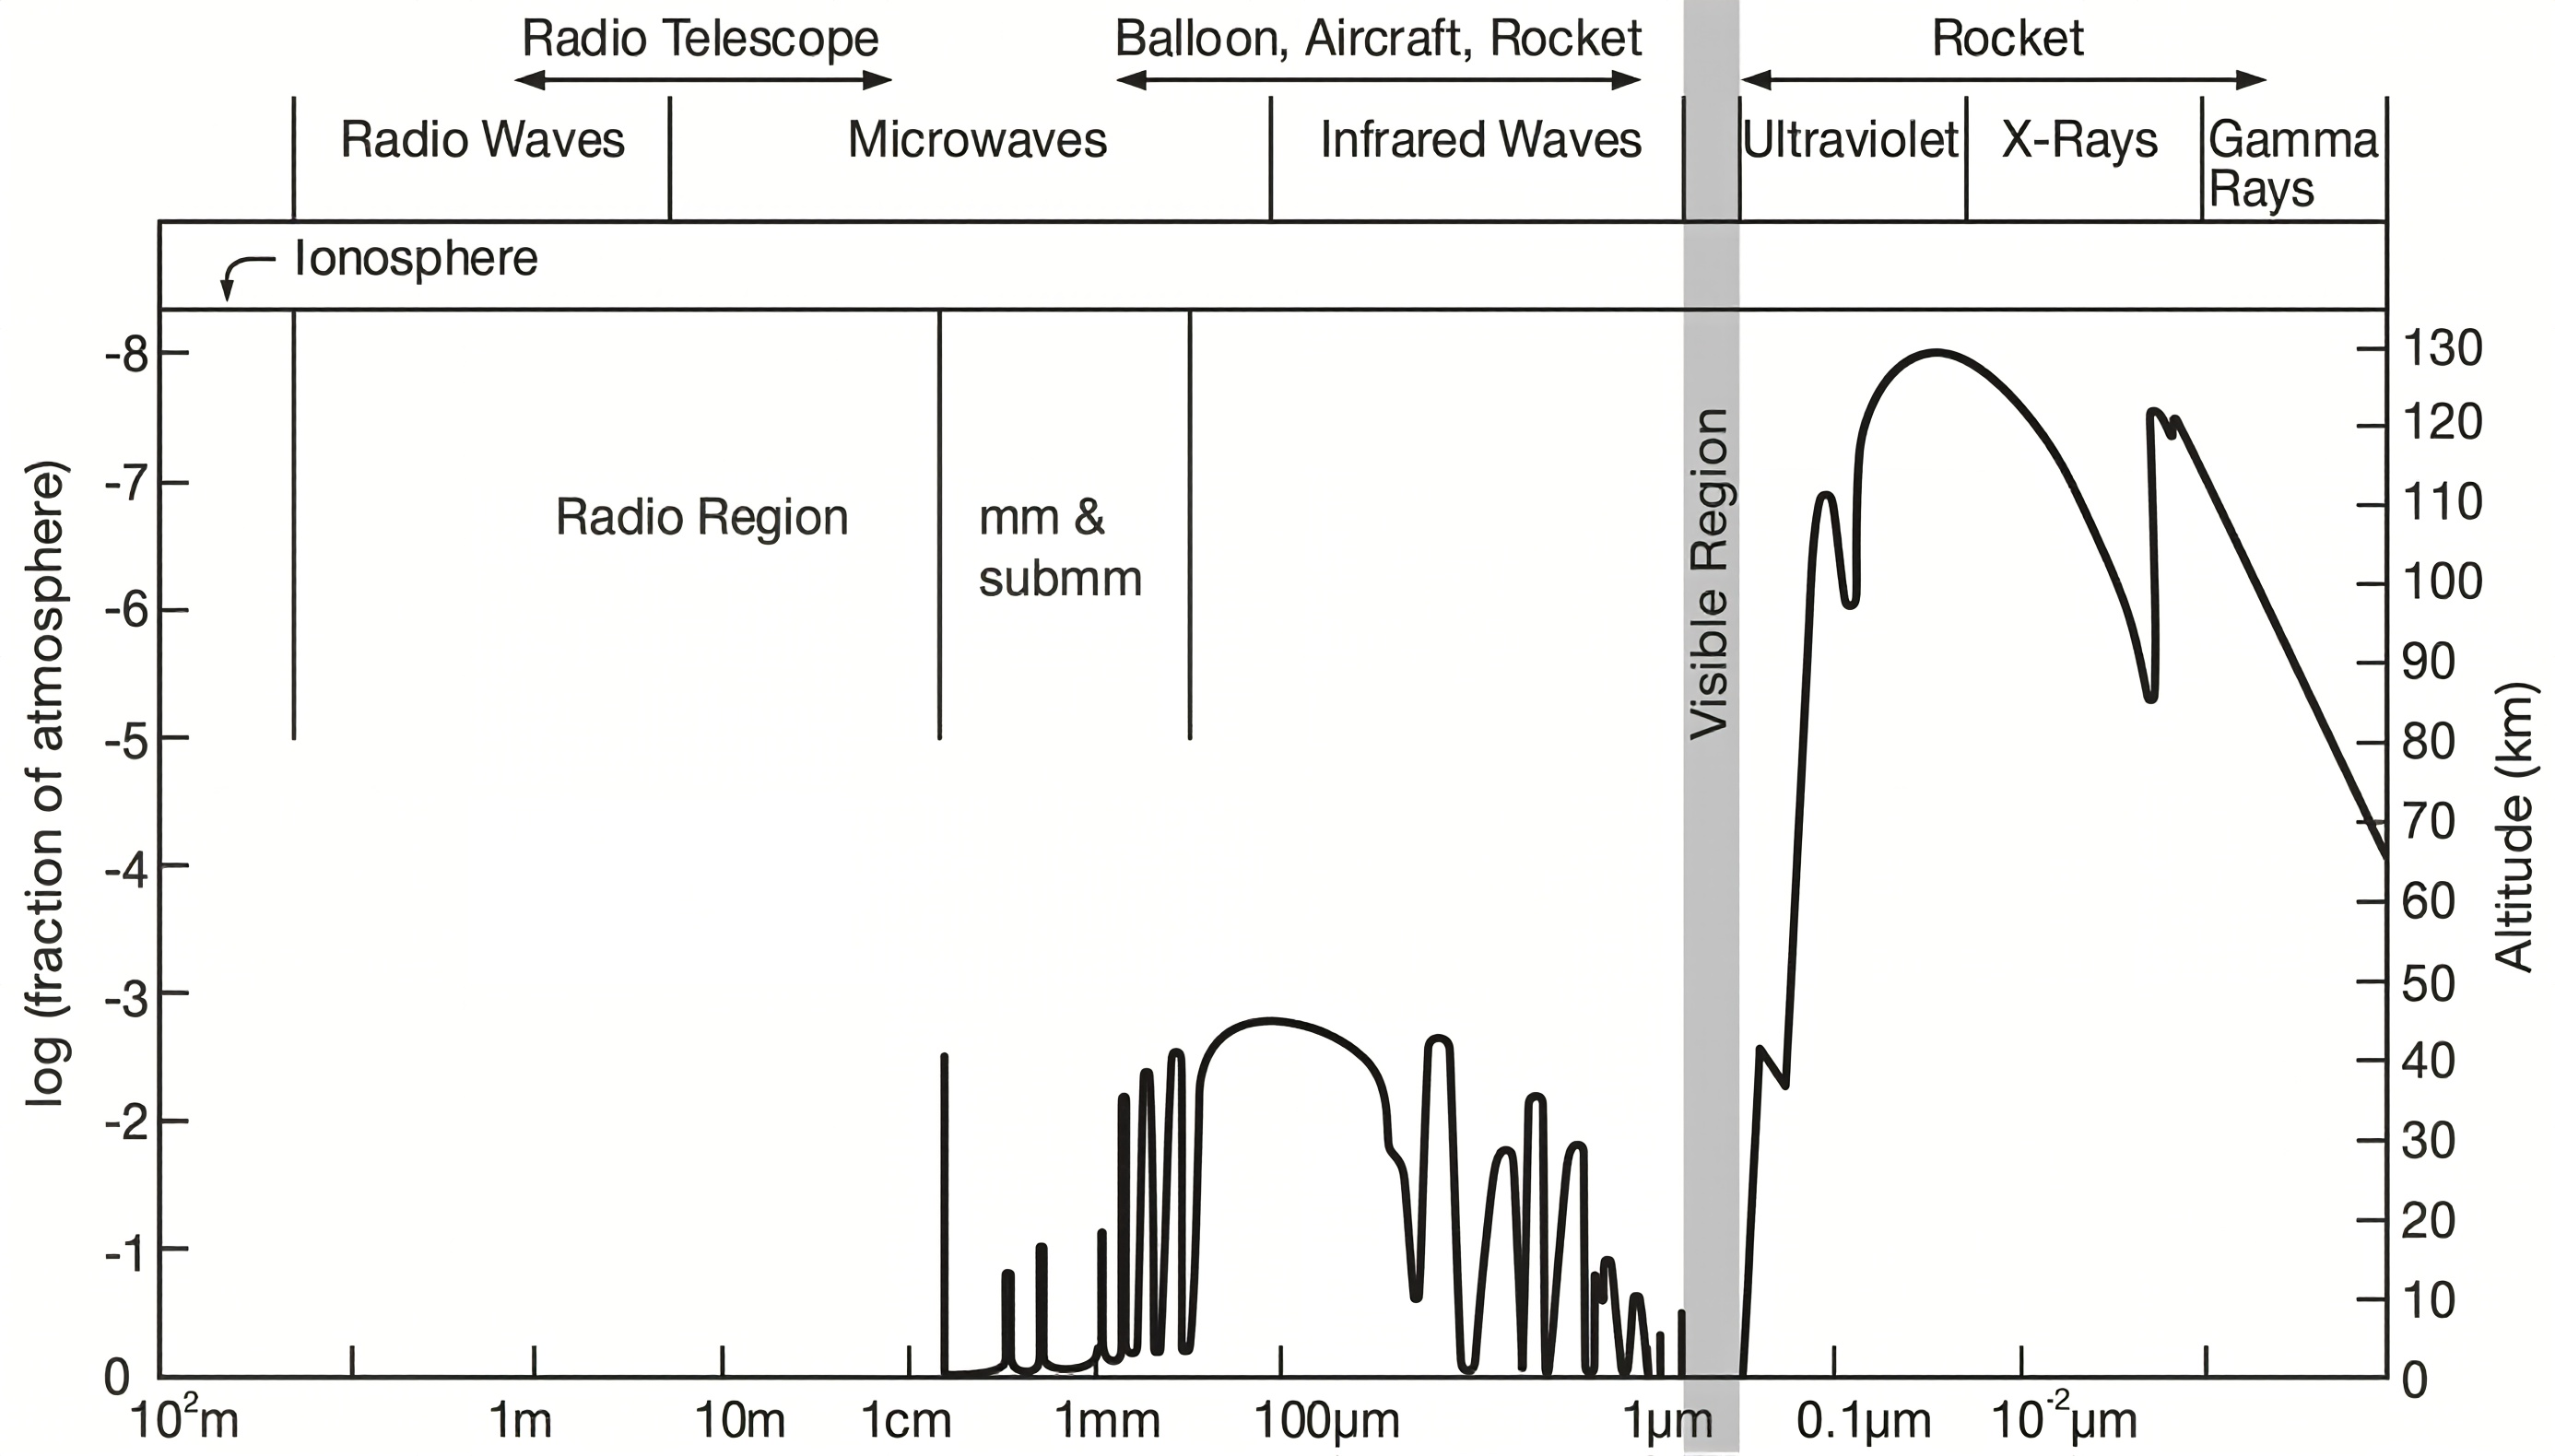
\includegraphics[width=0.85\textwidth]{assets/atmosphere_trasmission.png}
%     \caption{Atmosphere transmission}
%     \label{fig:atmosphere_transmission}
% \end{figure}

% Some objects as AGN are visible in all the frequency bands, other ones are visible only in some specific bands:

% \begin{itemize}
%     \item \textbf{Radio}: galaxies, AGN, pulsars, supernova remnants (SNR), $HI$
%     \item \textbf{mm/sub-mm}: Galaxy, CMB, dust, molecular clouds
%     \item \textbf{IR (FIR, MIR, NIR)}: dust, molecular clouds, K-M stars
%     \item \textbf{Optical/NUV}: stars, AGN, $HII$ regions
%     \item \textbf{UV-X}: $HII$ regions, stellar coronae, galaxy clusters, pulsars, X-ray binaries, AGN, SNR
%     \item \textbf{$\bm{\gamma}$}: most energetic events - Gamma-ray bursts (GRB), AGN, pulsars
% \end{itemize}

% \subsubsection{Information content of radiation}

% Multiple informations can be obtained from radio observations:

% \begin{itemize}
%     \item \textbf{Flux}: the rate of arriving photons, which provides constraints on \emph{luminosity} given assumptions about emission geometry. \emph{Periodicity} or \emph{variability} of the sources reveals its physical nature.
%     \item \textbf{Arrival direction/shape}: \emph{resolved} versus \emph{unresolved} sources (diffraction limit and atmospheric effects), and the nature of resolved sources.
%     \item \textbf{Spectrum}: the photon energy distribution reveals \emph{composition of source} (atomic features), \emph{temperature} (blackbody or bremsstrahlung), and line of sight \emph{relative velocity} or \emph{redshift}.
% \end{itemize}

% \subsection{Optical/UV and IR telescopes}

% \subsubsection{Image formation}

% we can suppose that photons from a distant object are parallel. The light is focused to a point in the focal plane.

% \begin{minipage}{0.45\textwidth}
%     The image dimensions are defined by:
%     \begin{itemize}
%         \item \textbf{Lens diameter}: $d$
%         \item \textbf{Focal length}: $f$
%     \end{itemize}
% \end{minipage}%
% \hfill
% \begin{minipage}{0.53\textwidth}
%     \centering
%     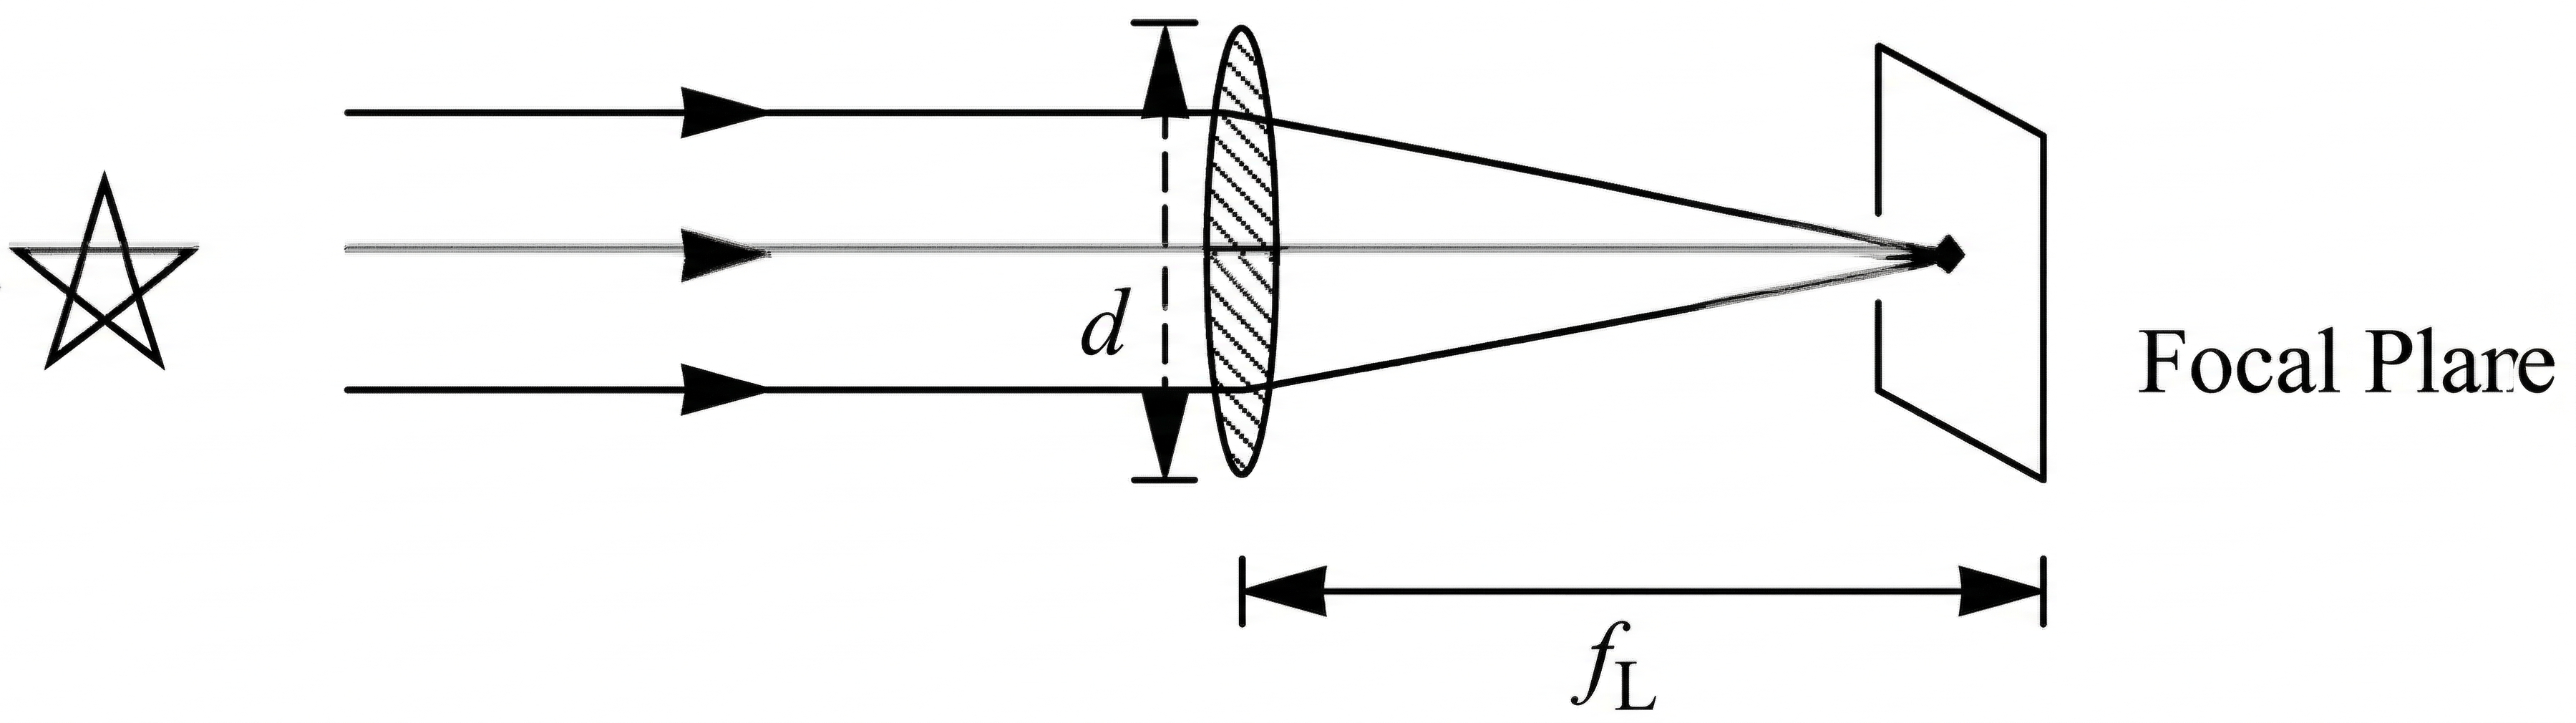
\includegraphics[width=\textwidth]{assets/image_formation.png}
%     % \captionof{figure}{Image formation}
% \end{minipage}

% The \textbf{Focal ratio} is the ratio between focal length and lens diameter:

% $$
% R = \dfrac{f}{d}
% $$

% \begin{itemize}
%     \item Low $R$ (~4-5) - Fast optical systems: Good to detect extended, low surface brightness objects, since they focus the light on a small surface of the detector (focal plane irradiance: $E_p \times \frac{1}{R}$ [W/m$^2$])
%     \item High $R$ (~10-15) - Slow optical systems: more suited for high-resolution observations
% \end{itemize}

% \begin{minipage}{0.5\textwidth}

% Focal point varies with angle of incoming light:
% $$
% s = \tan \alpha f_L \approx \alpha f_L
% $$

% We can then define the \textbf{plate scale} as:

% \end{minipage}
% \hfill
% \begin{minipage}{0.48\textwidth}
%     \centering
%     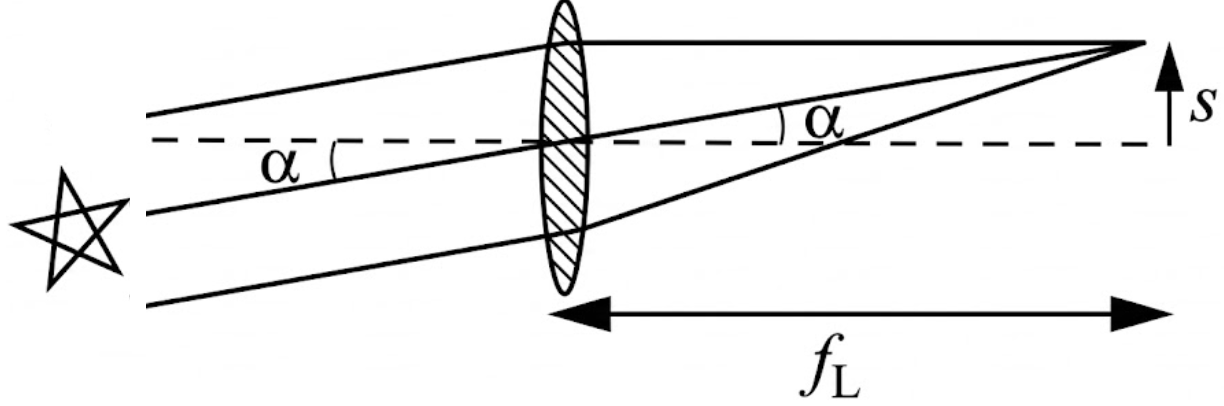
\includegraphics[width=\textwidth]{assets/image_formation_2.png}
%     % \captionof{figure}{Focal point variation}
% \end{minipage}
 
% $$
% \text{PS} = \dfrac{\alpha}{s} = \dfrac{1}{f_L}
% $$

% The plate scale is related to the Field of View (FoV) as:

% $$
% \theta_{max} = \arctan \left( \dfrac{d/2}{f_L} \right) \qquad \text{FoV} = 2 \arctan \left( \dfrac{d/2}{f_L} \right) \approx \dfrac{d}{f_L} \qquad \Rightarrow \text{PS} = d \cdot \text{FoV}
% $$

% \subsubsection{Fast and slow optical systems}

% Fast and slow optical systems differ by their \textbf{focal ratio}:

% \begin{itemize}
%     \item \textbf{Fast systems} (low $R$): Deliver higher irradiance per unit area on the detector and are optimal for extended, low surface brightness imaging (wide field surveys).
%     \item \textbf{Slow systems} (high $R$): Provide higher angular magnification and are better suited for point-source and high-resolution applications.
% \end{itemize}


% \begin{table}[h]
%     \centering
%     \renewcommand{\arraystretch}{1.3}
%     \begin{tabular}{@{} l c c @{}}
%         \toprule
%         \textbf{Characteristic} & \textbf{James Webb (JWST)} & \textbf{Euclid} \\
%         \midrule
%         Mirror Diameter & 6.5 m & 1.2 m \\
%         Focal Length & $\sim$131 m & 24.5 m \\
%         Focal Ratio & 20 & 20 \\
%         Field of View (FoV) & Very narrow: $\sim$arcmin (Detail) & Very wide: 0.57 deg$^2$ (Survey) \\
%         Cosmological Objective & First stars and galaxies (depth) & Dark Matter/Energy (statistics) \\
%         \bottomrule
%     \end{tabular}
%     \caption{Comparison between JWST and Euclid}
%     \label{tab:jwst-euclid-comparison}
% \end{table}

% \begin{observationblock}[FoV and focal ratio]
% Although JWST and Euclid share the same focal ratio ($R = 20$), their fields of view differ dramatically. This apparent paradox is resolved by understanding that the FoV depends on the \textbf{detector size}, not just the focal ratio. Euclid achieves its wide field of view by employing a large mosaic of detectors at its focal plane, effectively increasing the physical size $d$ of the detection area. Since $\text{FoV} \approx d/f_L$, a larger detector array directly translates to a wider field of view, even when the focal ratio remains constant.
% \end{observationblock}

% \subsection{Telescope configurations}

% % brief introduction to telescope configurations

% \subsubsection{Refracrot Telescopes}

% Refractor telescopes use \textbf{lenses} to focus the light.

% \begin{itemize}
%     \item Pro: Aberration reduced or eliminated (beyond notice) using aspherical, achromatic, multiple lenses at objective and eyepiece.
%     \item Cons:
%     \begin{itemize}
%         \item large lenses are heavy and
%         deform under their own weight;
%         \item chromatic aberration cannot be
%         eliminated;
%         \item light absorbed by lens to achieve large f/ numbers, telescope is long and so requires massive supports and large domes;
%     \end{itemize}
% \end{itemize}

% \subsubsection{Reflecting Telescopes}

% Reflecting telescopes use \textbf{mirrors} to focus the light.

% \begin{itemize}
%     \item Pro:
%     \begin{itemize}
%         \item mirror can be supported from the back and gravitational deformations corrected using active optics;
%         \item no chromatic aberration;
%         \item mirrors can have higher reflectivity than lenses have transparency;
        
%         \item by having multiple reflections inside telescope tube, telescope can be shorter to achieve same f/ number and so requires less massive supports and domes;
%     \end{itemize}
% \end{itemize}

% \begin{figure}[H]
%     \centering
%     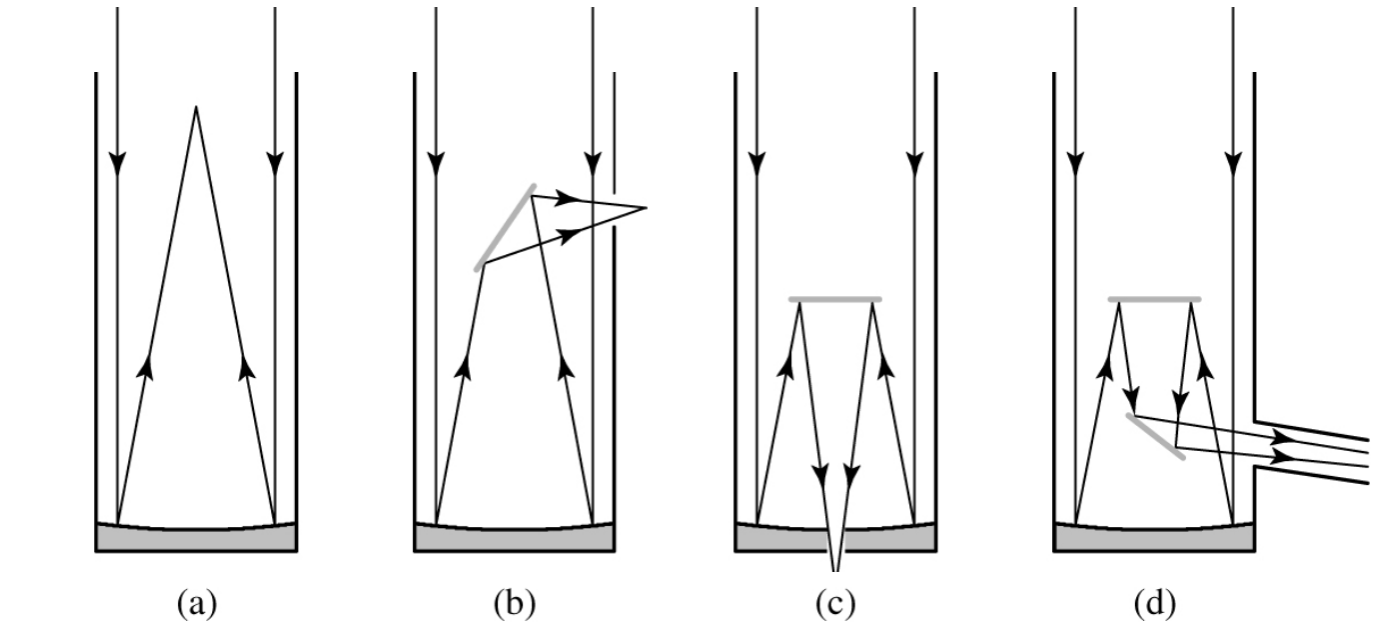
\includegraphics[width=0.6\textwidth]{assets/reflectors_config.png}
%     \caption{(a) Primary focus (b) Newtonian (c) Cassegrain (d) Nasmyth/Coudè}
%     \label{fig:reflectors_configurations}
% \end{figure}

% (a) Wide-field camera are deployed at the prime focus as to have the shortest focal length

% (b-c) If the secondary mirror is curved rather than flat, the focal length of the telescope can be changed

% (d) Coudé (or Nasmyth) focus has a very long focal length and uses an additional mirror to transport the focus to a nearby instrument, typically a very stable spectrograph in a temperature controlled room

% \subsection{Optical/NIR detectors}

% % what are detectors? write brief introduction

% \subsubsection{Photographic plates}

% Photographic plates have been used to image the sky and obtain spectra of astrophysical sources over the past century:

% \begin{itemize}
%     \item A light sensitive emulsion is applied to glass plates
%     \item Plates are exposed and each absorbed photon results in a chemical change in a molecule of this emulsion
%     \item Plates are then developed in a chemical process
% \end{itemize}

% Plates have a non-linear response, because the probability of detecting an incoming photon depends on the density of light-sensitive chemicals in plate. As light is absorbed this density falls and the plate becomes less sensitive.

% \subsubsection{CCD detectors}

% A Charge Coupled Device (CCD) is a 2D array of silicon pixels that converts incoming photons into stored electric charge. Each pixel acts as a potential well for photo-electrons.

% CCD surface is divided into rows and columns of pixels with characteristic size $\sim 10 \mu$m; typical sizes are 2048 to 4096 on a side, corresponding to $\sim$2.5 cm.

% High linearity and broad wavelength sensitivity have made CCDs the detector of choice in optical astronomy.

% Nowadays large sky cameras are built from large arrays of CCDs, enabling efficient mapping of large portions of the sky.

% \begin{figure}[H]
%     \centering
%     \begin{minipage}{0.55\textwidth}
%         \centering
%         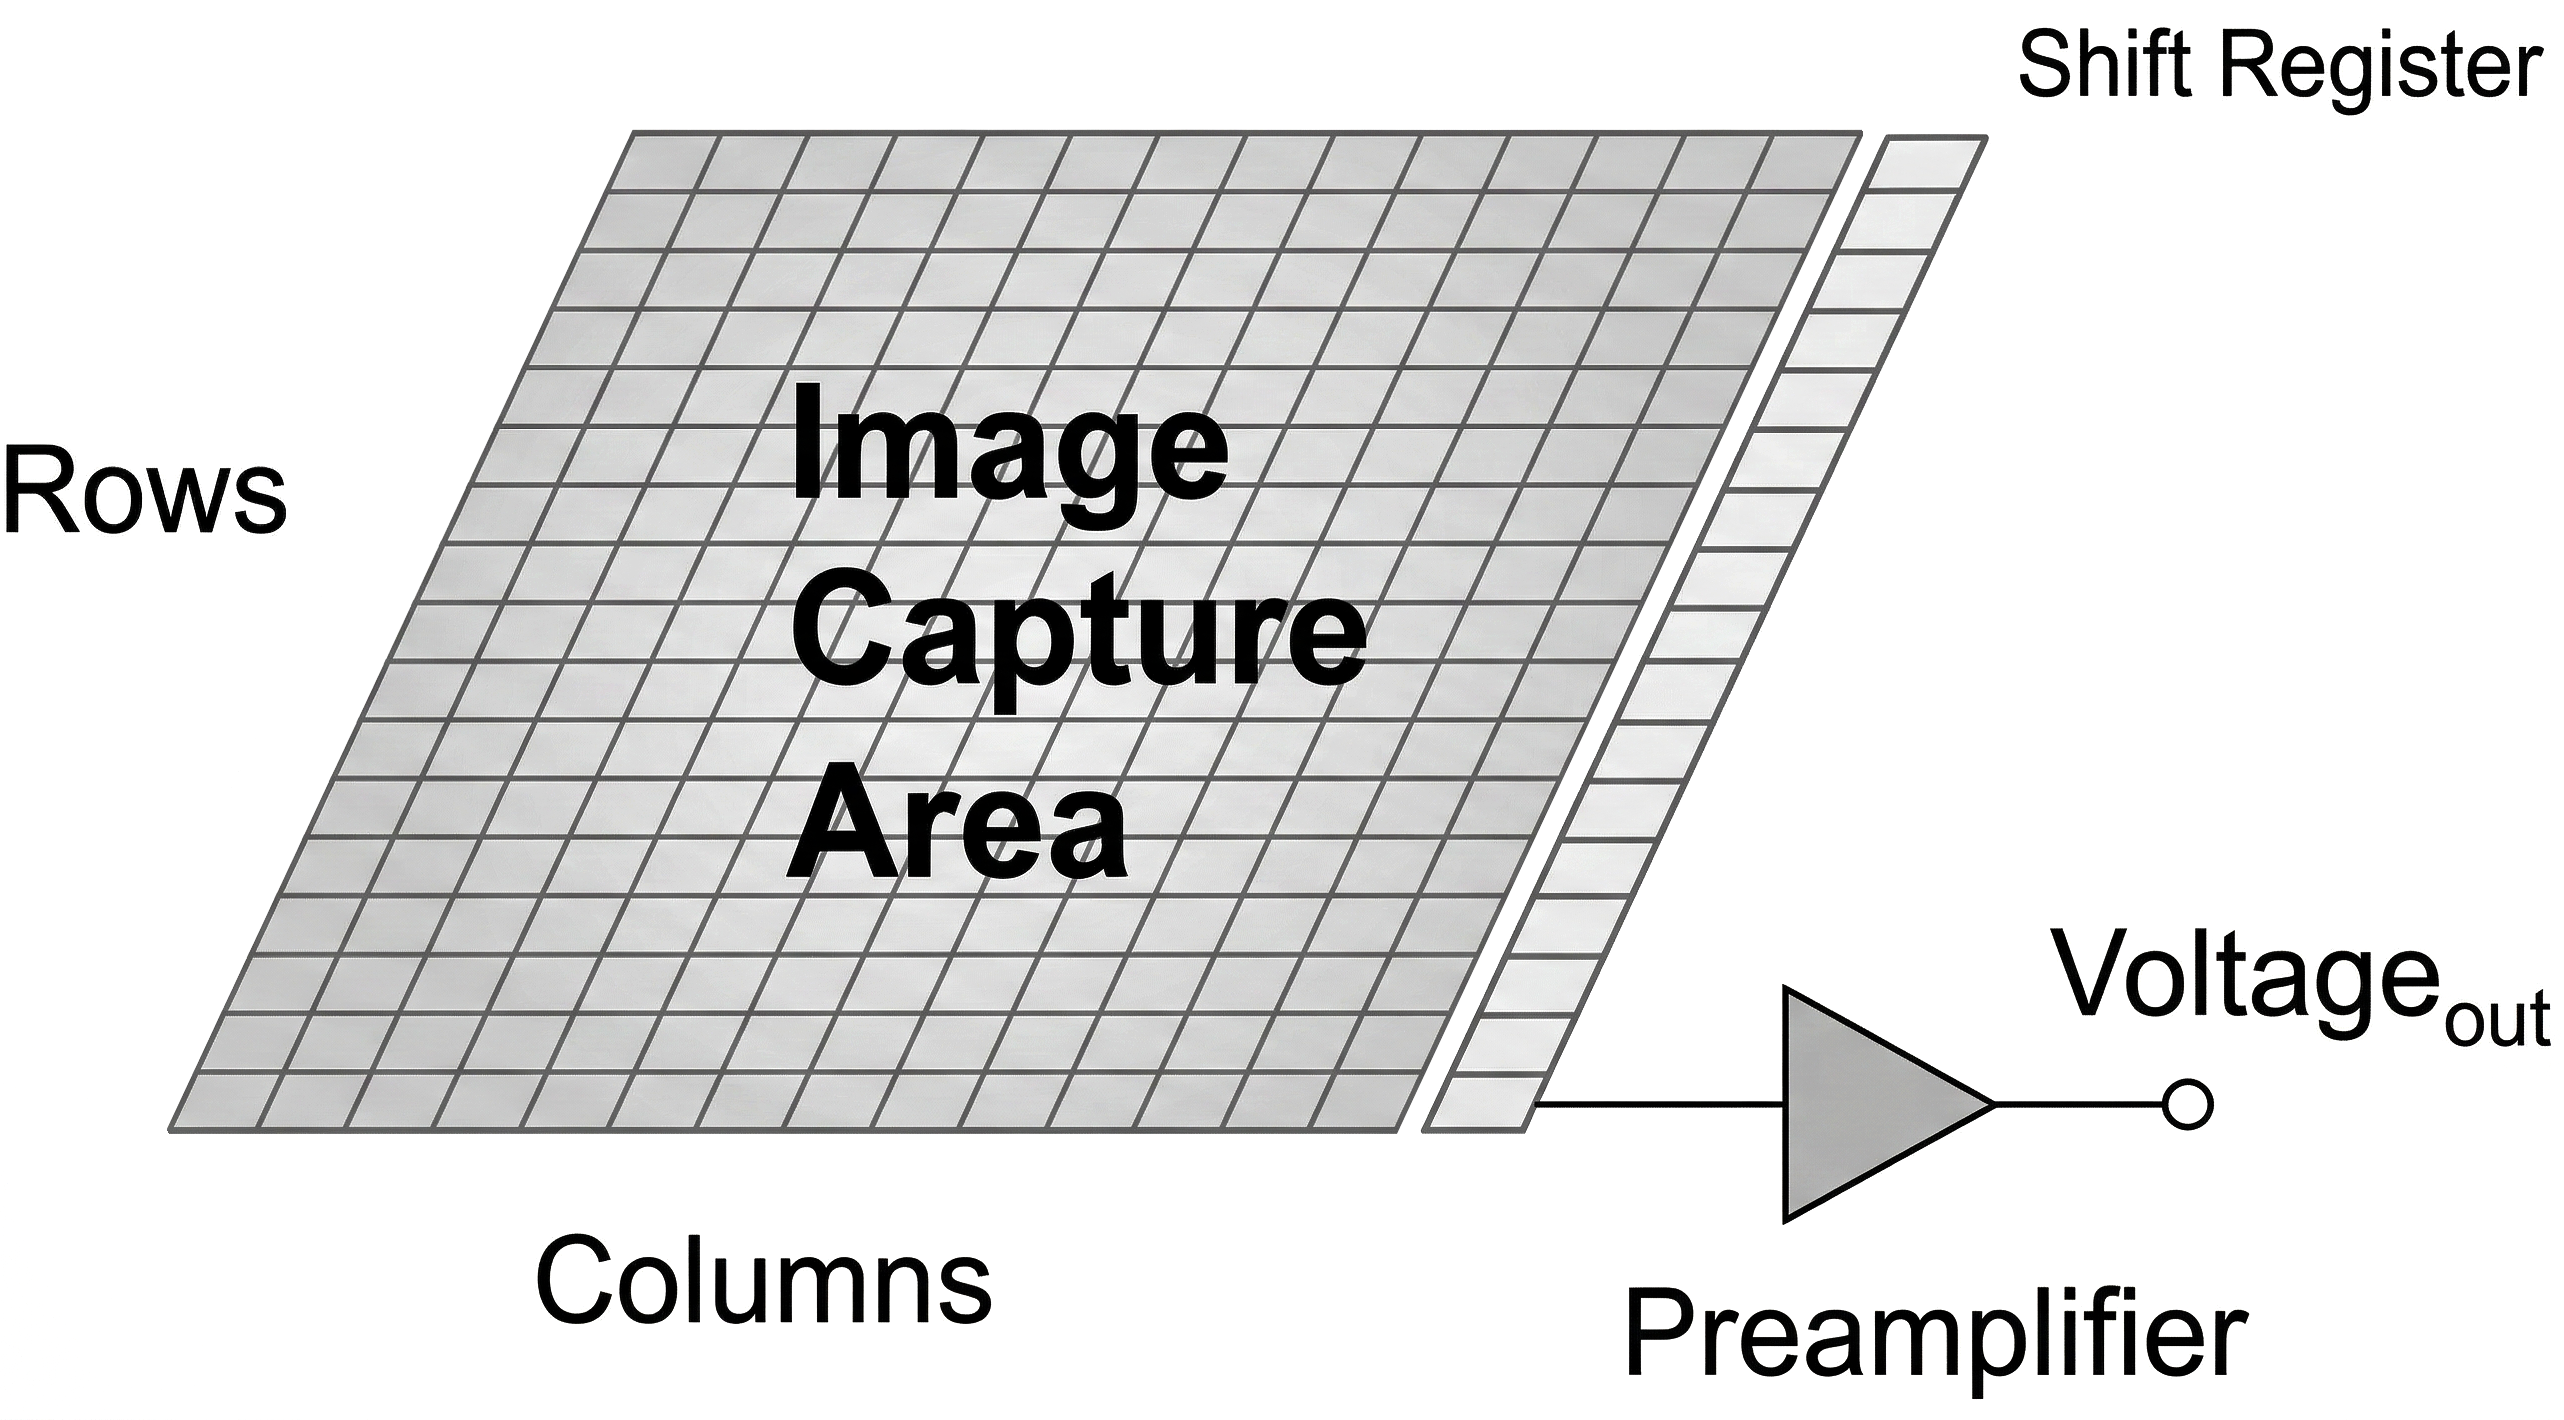
\includegraphics[width=0.8\textwidth]{assets/ccd.png}
%         \captionof{figure}{\textbf{Left}: Schematic of a CCD. \textbf{Right}: Rain bucket analogy: photons (rain) fall into pixel wells arranged in vertical columns; during readout, accumulated charge is shifted row by row into a horizontal serial register, then measured at the output node.}
%     \end{minipage}
%     \hfill
%     \begin{minipage}{0.43\textwidth}
%         \centering
%         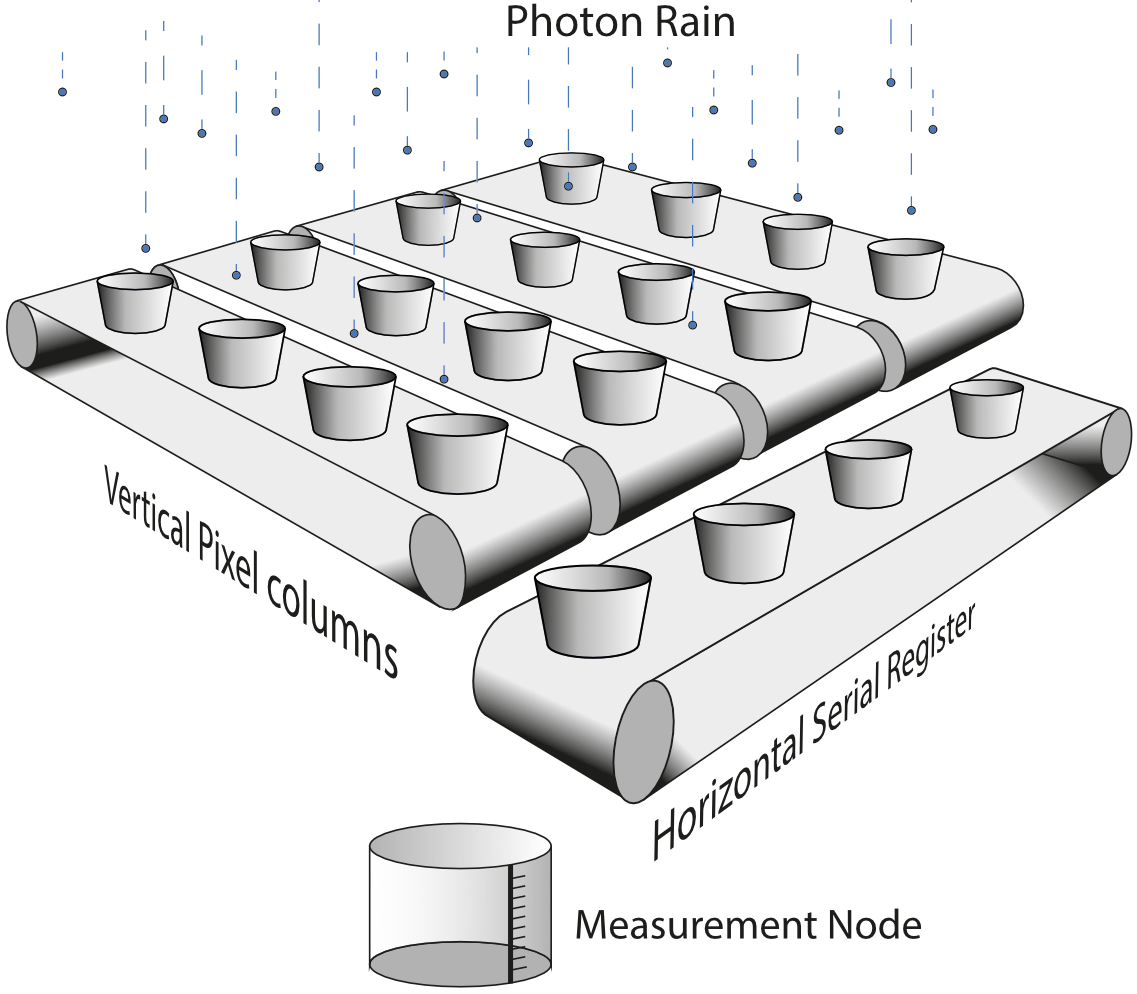
\includegraphics[width=\textwidth]{assets/ccd_analogy.png}
%     \end{minipage}
%     \label{fig:ccd_analogy}
% \end{figure}

% CCDs are:

% \begin{itemize}
%     \item Extremely sensitive with quantum efficiencies $\text{QE} = \frac{\text{\# }e^- \text{ collected}}{\text{\# incoming } \gamma}$ reaching 80\% or higher
%     \begin{itemize}
%         \item For comparison photographic plates or eye have QE $\sim$ 1\%
%     \end{itemize}
%     \item Sensitive to photons over a broad range of energies ($>1.11$eV or $<1.1 \mu$m, the silicon band gap)
%     \item Have a linear response over dynamic range of $10^5$ (read noise floor of 1-2 $e^-$ and full well capacity of $\sim 10^5$ $e^-$)
%     \begin{itemize}
%         \item Compare to photographic plates that are linear over dynamic range of $10^2$
%     \end{itemize}
% \end{itemize}

% These properties allow:

% \begin{itemize}
%     \item Quantitative astrometric measurements of extended sources
%     \item Time-domain astronomy
%     \item Wide-field surveys
%     \begin{itemize}
%         \item E.g. Sloan Digital Sky Survey, Pan-STARRs1, Dark Energy Survey, Euclid, LSST
%     \end{itemize}
% \end{itemize}

% \begin{minipage}{0.7\textwidth}
%     Raw images from a given CCD typically
%     have unwanted structures:

%     \begin{itemize}
%         \item Read-outs might have different bias level
%         \item Saturation or spikes around bright sources
%         \item Electronic artifacts, e.g. dead or bright columns
%         \item In addition to cosmic rays, scattered light, satellite trails, etc.
%     \end{itemize}

%     \medskip

%     Single epoch (exposure) images need to be calibrated to remove all these effects.
    
%     Coadded images are science ready data which combine calibrated single epoch images to create high quality images.
% \end{minipage}%
% \hfill
% \begin{minipage}{0.28\textwidth}
%     \centering
%     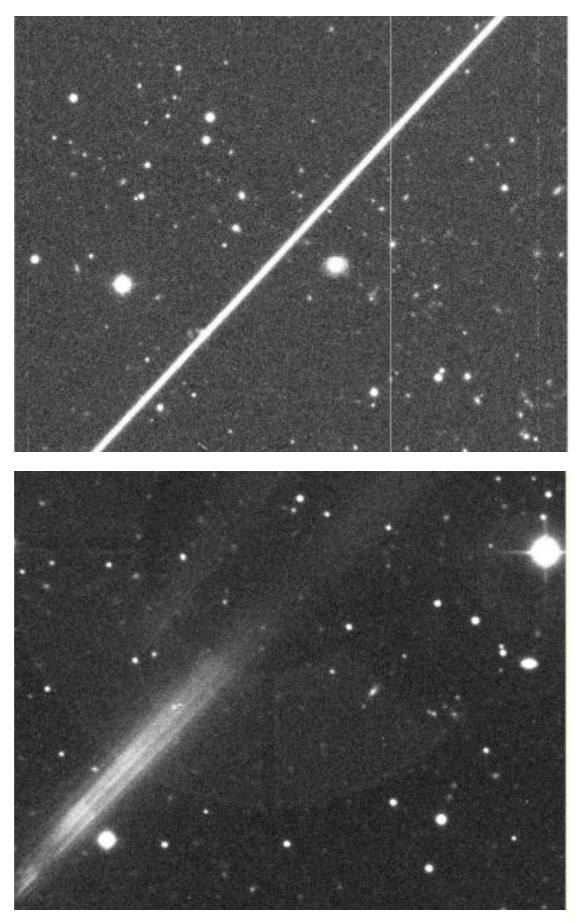
\includegraphics[width=0.9\textwidth]{assets/ccd_artifacts.png}
% \end{minipage}

% \subsubsection{CMOS detectors}

% CMOS detectors are solid-state imaging arrays where each pixel contains its own readout electronics, i.e. charge is converted to voltage locally, not shifted across the array.

% \begin{itemize}
%     \item Each pixel includes:
%     \begin{itemize}
%         \item Charge-to-voltage converter
%         \item Amplifier
%     \end{itemize}
%     \item No charge transfer across the detector
%     \item High readout speed
% \end{itemize}

% CMOS couple photodiode made from material that is photosensitive at the desired wavelength (HgCdTe) to a silicon readout circuit (Hybrid devices).

% Sensitivity to low energy photons then requires low operating temperatures ($<100$ K) to suppress thermal noise (or dark current).

% \begin{figure}[H]
%     \begin{minipage}{0.5\textwidth}
%         \centering
%         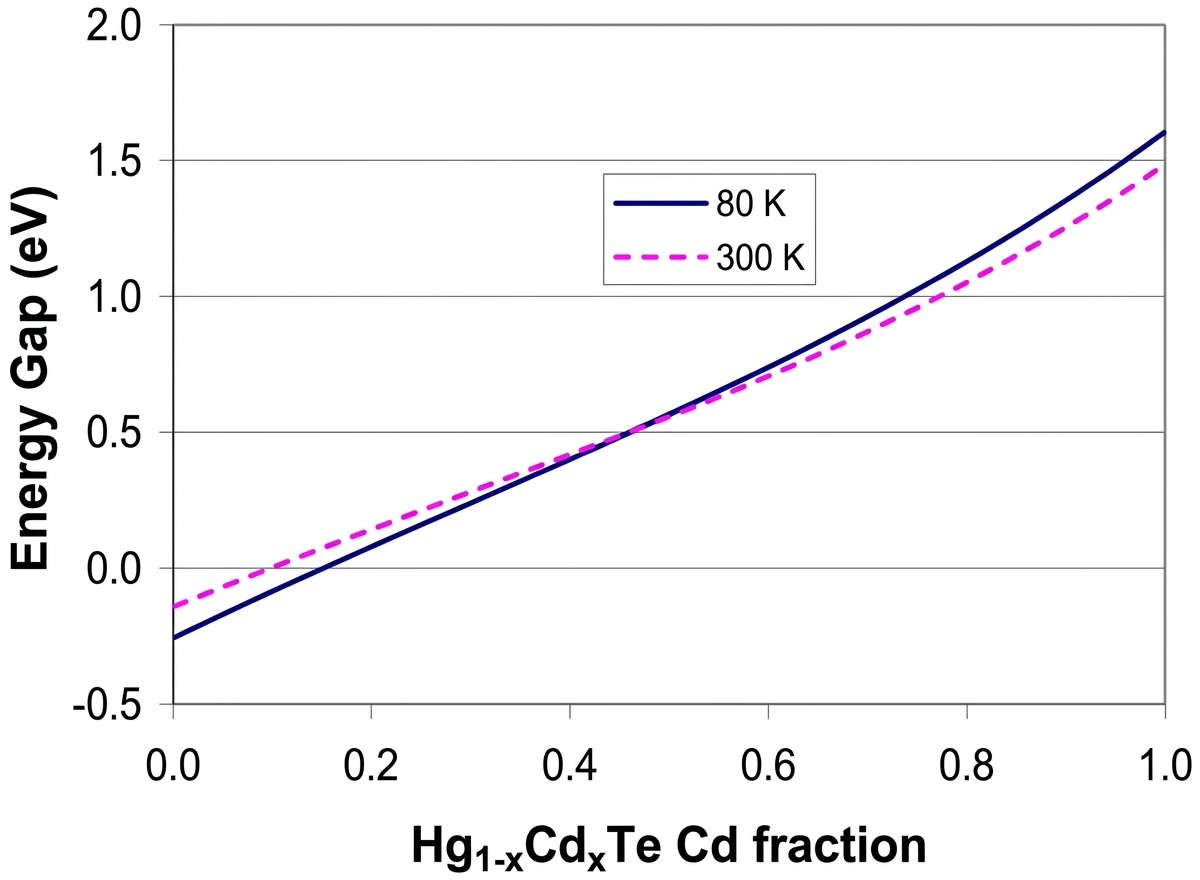
\includegraphics[width=\textwidth]{assets/cmos.png}
%     \end{minipage}%
%     \hfill
%     \begin{minipage}{0.48\textwidth}
%         \caption{HgTe is a semimetal and CdTe is a semiconductor. By adjusting the Cd fraction one can tune the wavelength sensitivity of the HgCdTe arrays. The plot shows the energy gap as a function of Hg$_{1-x}$Cd$_x$Te Cd fraction at different temperatures.}
%         \label{fig:cmos_hgcdte}
%     \end{minipage}
% \end{figure}

% \begin{minipage}{0.7\textwidth}
%     Ground based IR images look like noise:
%     \begin{itemize}
%         \item Observations are usually background limited: the sky is so bright in the IR band that the exposures must be very short ($\sim$10s)
%         \item Narrow atmospheric windows (J, H, K bands) due strong molecular absorption (H$_2$O, CO$_2$, CH$_4$)
%         \item Large series of images are taken with small dithers
%         \item Sky is subtracted and images coadded as with CCD images
%     \end{itemize}

%     \medskip

%     From space the background is much lower (dominated by zodiac light), but there is a higher particle background (cosmic rays).
% \end{minipage}%
% \hfill
% \begin{minipage}{0.28\textwidth}
%     \centering
%     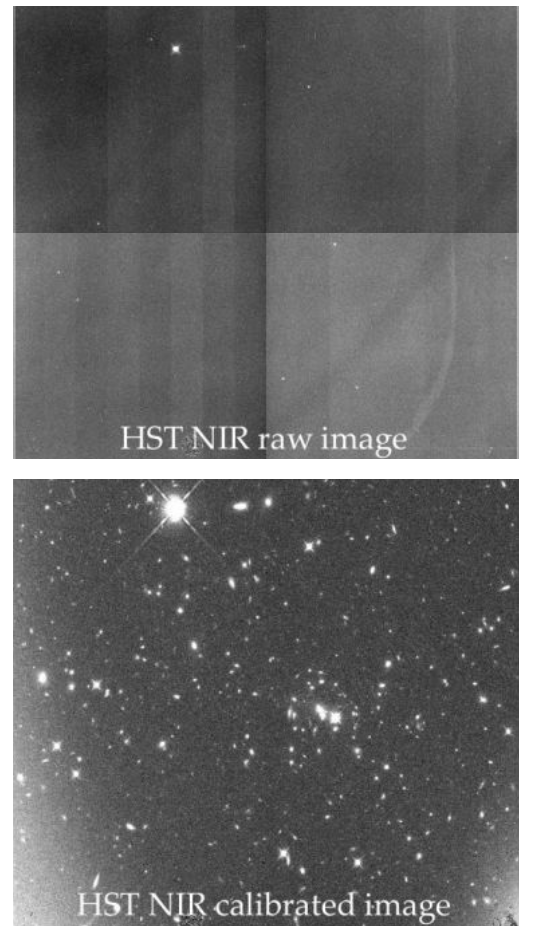
\includegraphics[width=\textwidth]{assets/cmos_artifacts.png}
% \end{minipage}

% \subsubsection{NIR}

% \textbf{Photometric Passbands:}

% \begin{itemize}
%     \item In optical and NIR photometry one often encounters measurements in particular passbands. The table on the right is a list of the standard broadband filters.
%     \item Narrow band filters are often used to seek particular spectral lines or features and/or improve constraints on the spectral energy distribution of the source.
% \end{itemize}

% \begin{figure}[H]
%     \begin{minipage}{0.45\textwidth}
%         \centering
%         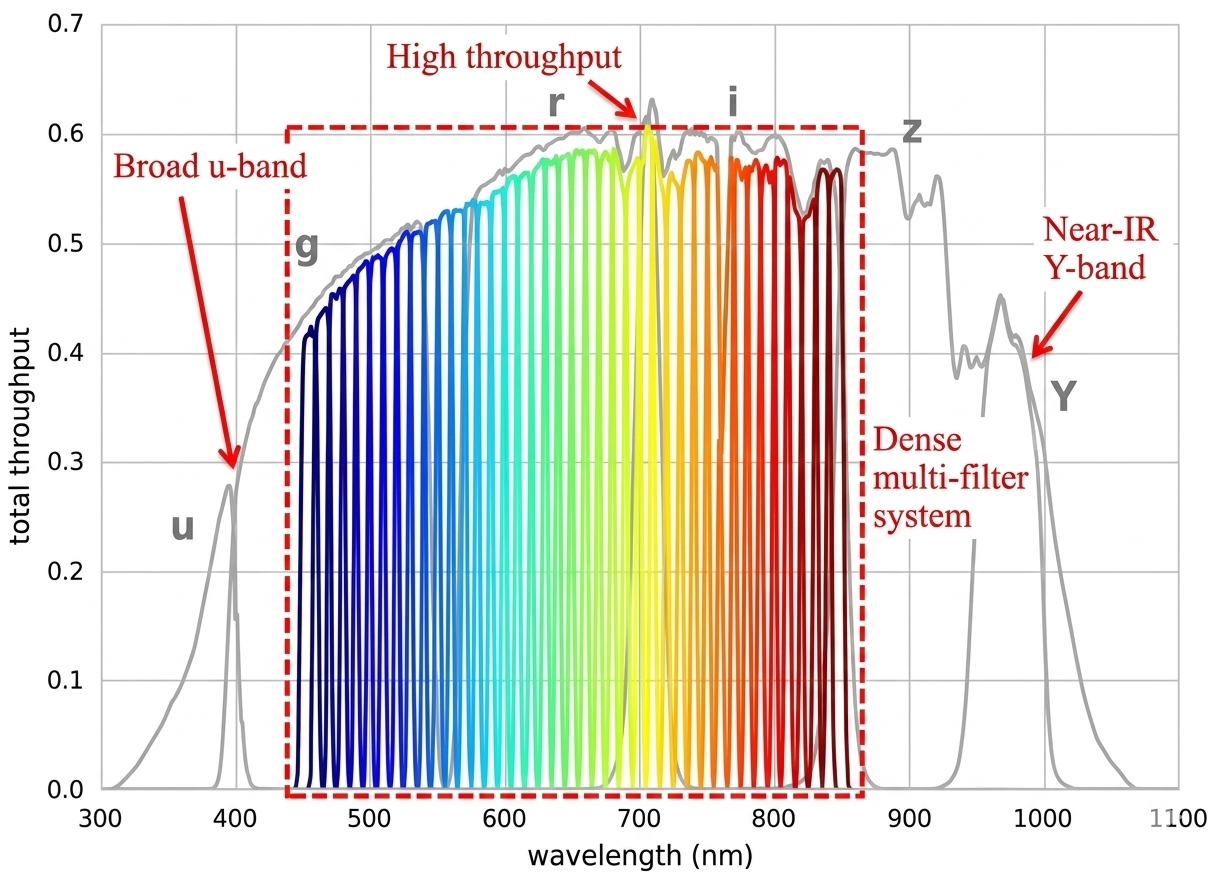
\includegraphics[width=\textwidth]{assets/pau_bands.png}
%         \caption{40 narrow bands of the PAU camera}
%         \label{fig:pau_bands}
%     \end{minipage}%
%     \hfill
%     \begin{minipage}{0.5\textwidth}
%         \centering
%         \begin{tabular}{c c c}
%             \toprule
%             Band & $\lambda_{\text{mid}}$ & $\Delta\lambda$ \\
%             \midrule
%             U & 365 & 66 \\
%             B & 445 & 94 \\
%             V & 551 & 88 \\
%             R & 658 & 138 \\
%             I & 806 & 149 \\
%             Z & 900 & \\
%             Y & 1020 & 120 \\
%             J & 1220 & 213 \\
%             H & 1630 & 307 \\
%             K & 2190 & 390 \\
%             L & 3450 & 472 \\
%             M & 4750 & 460 \\
%             \bottomrule
%         \end{tabular}
%     \end{minipage}
% \end{figure}

% \subsubsection{Optical/NIR: Ground vs Space}

% For space-based (or small ground-based) telescopes the angular resolution is limited by the diffraction of the telescope aperture.

% The diffraction pattern produced by a circular aperture is known as the Airy pattern, which comprises a bright central disk (83.3\% of the energy) surrounded by much dimmer diffraction rings.

% The first minima, which define the Airy disk, occurs at:
% $$
% \theta = 1.22 \frac{\lambda}{D}
% $$

% \begin{figure}[H]
%     \centering
%     \begin{minipage}{0.45\textwidth}
%         \centering
%         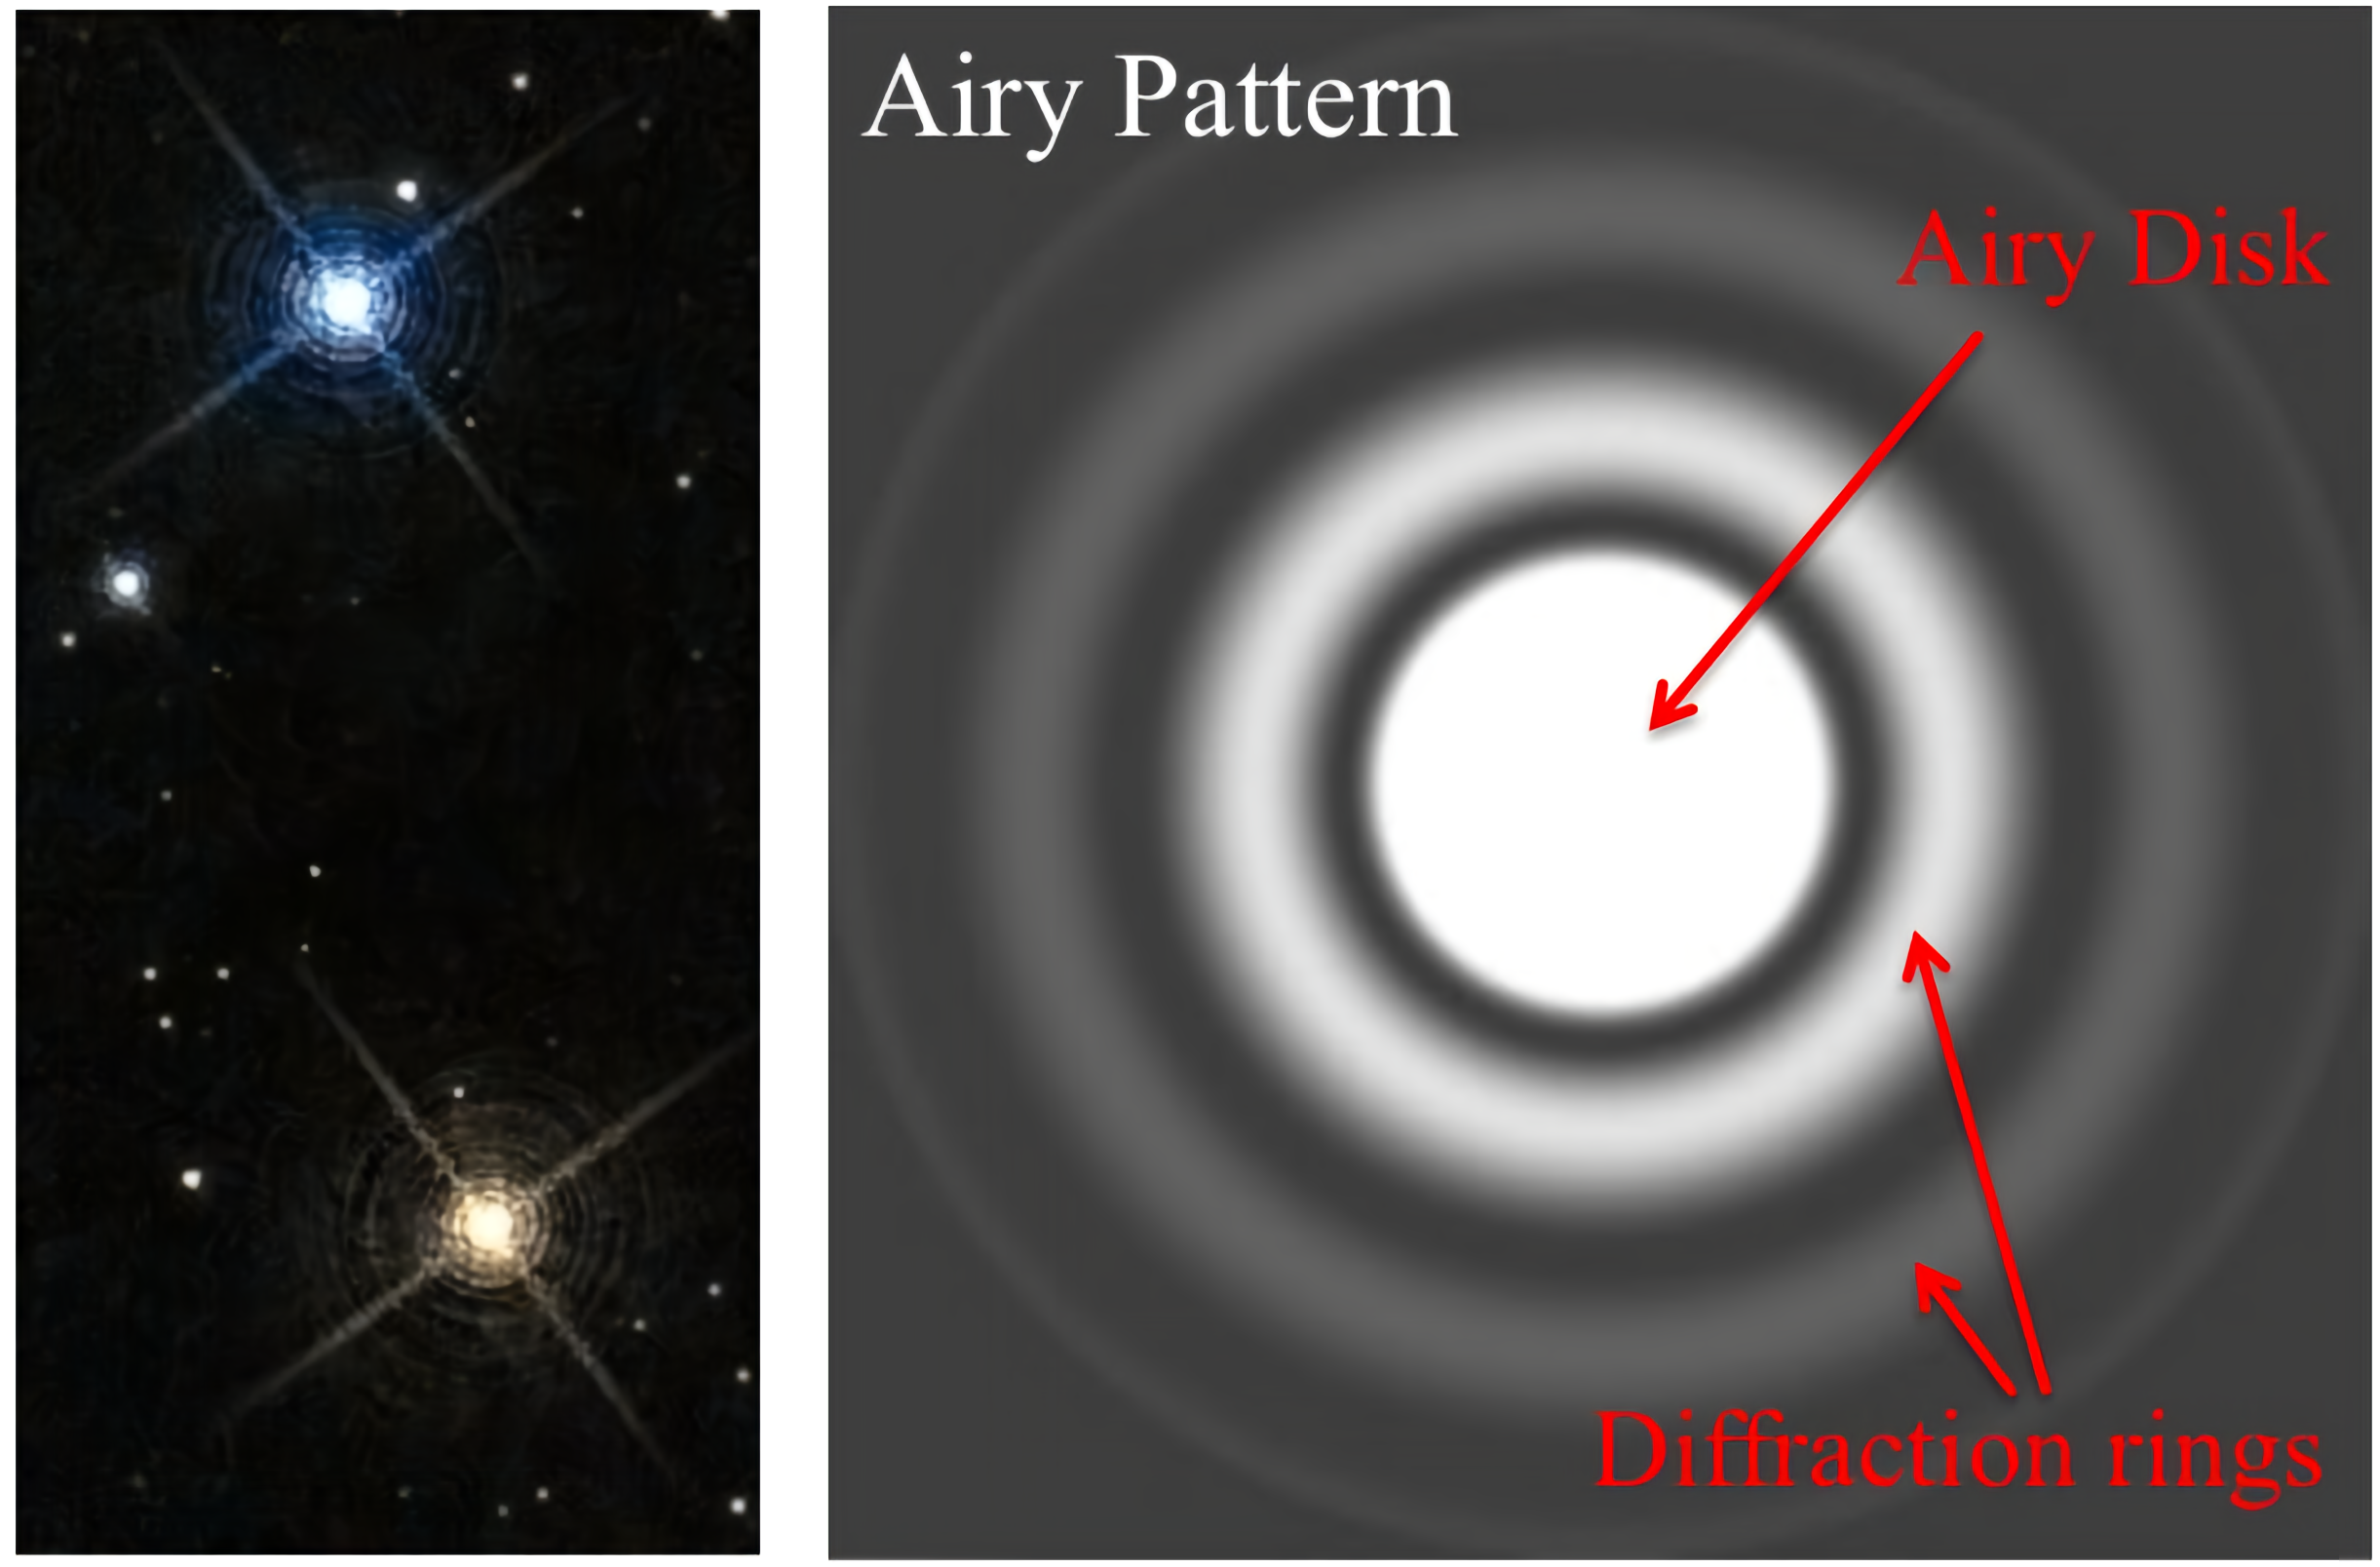
\includegraphics[width=\textwidth]{assets/airy_effect.png}
%     \end{minipage}%
%     \hfill
%     \begin{minipage}{0.53\textwidth}
%         \centering
%         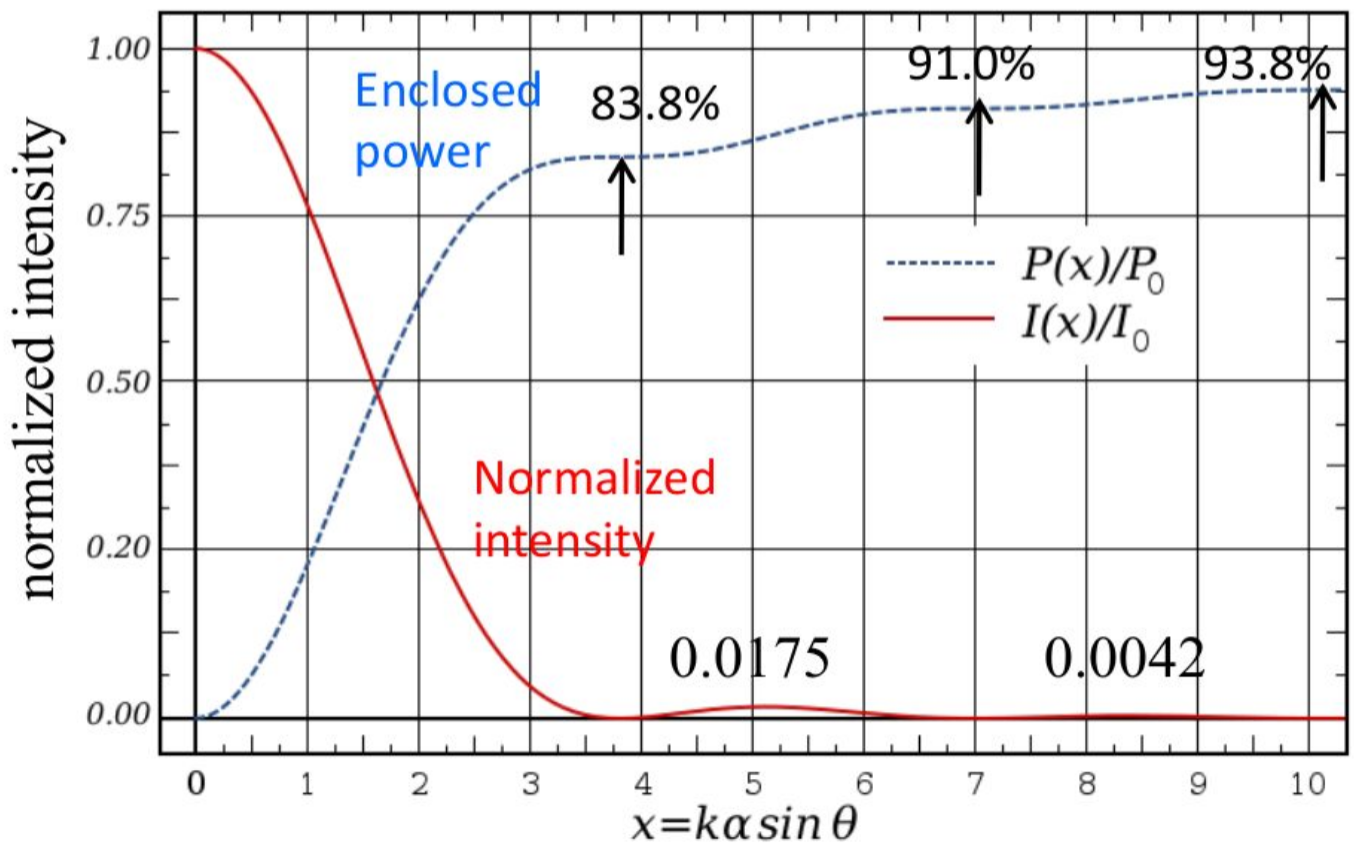
\includegraphics[width=\textwidth]{assets/intensity.png}
%     \end{minipage}
%     \caption{Airy diffraction pattern}
%     \label{fig:airy_effect}
% \end{figure}

% The \textbf{Rayleigh criterion} for resolving two point sources requires:
% $$
% \Delta\theta > 1.22 \frac{\lambda}{D}
% $$

% The Rayleigh criterion corresponds closely to the diameter of the Airy disk as measured at full-width half-maximum (FWHM), which provides a more convenient measure of the angular resolution.

% Angular resolution at optical wavelengths (0.5 $\mu$m) of human eye at night is about 20".

% \begin{itemize}
%     \item 2.4 m, $\theta_{\text{min}} = 0.05''$ (Hubble Space Telescope)
%     \item 4 m, $\theta_{\text{min}} = 0.03''$ (Canada-France-Hawaii Telescope)
%     \item 8.2 m, $\theta_{\text{min}} = 0.015''$ (Subaru Telescope)
% \end{itemize}

% For large ground-based telescopes the Point-Spread Function (PSF) is a function of atmosphere, rather than telescope optics.

% The PSF is well described by a Moffat profile with free parameters $R$ (width) and $\beta$ (shape):
% $$
% I(r) = \frac{I_0}{(1 + r^2/R^2)^\beta} + B
% $$

% The ``seeing'' disk, which defines the resolution of ground-based telescopes, corresponds to the FWHM of the PSF. A seeing of 0.5'' is very good, 2'' is bad (e.g. weak lensing measurements require $< 1''$). Without corrections all telescopes with $D > 25$ cm are limited by atmospheric seeing $\rightarrow$ adaptive optics.

% \subsection{Optical/NIR: Telescopes}

% \subsubsection{ELT}

% The \textbf{Extremely Large Telescope} (ELT) is the European Southern Observatory's flagship ground-based telescope currently under construction in Chile:

% \begin{itemize}
%     \item \textbf{Primary mirror}: 39 m (segmented, 798 hexagonal segments)
%     \item \textbf{Field of View}: 10 arcmin
%     \item \textbf{Adaptive optics}: Advanced system with 6 laser guide stars
%     \item \textbf{Instrumentation}: 2 Nasmyth platforms
%     \item \textbf{First light}: Expected 2029
% \end{itemize}

% \subsubsection{JWST}

% The \textbf{James Webb Space Telescope} (JWST) is a NASA/ESA/CSA infrared space observatory:

% \begin{itemize}
%     \item \textbf{Primary mirror}: 6.5 m (segmented, 18 hexagonal gold-coated beryllium segments)
%     \item \textbf{Field of View}: $\sim$4 arcmin
%     \item \textbf{Instruments}: NIRCam, NIRSpec, MIRI (MIR camera/spectrograph), FGS/NIRISS
%     \item \textbf{Wavelength range}: 0.6--28.5 $\mu$m
%     \item \textbf{Location}: L2 Lagrange point
%     \item \textbf{Launched}: December 2021
% \end{itemize}

% \subsubsection{Euclid}

% \textbf{Euclid} is an ESA space mission designed to study dark energy and dark matter:

% \begin{itemize}
%     \item \textbf{Primary mirror}: 1.2 m
%     \item \textbf{Field of View}: $\sim$0.5 deg$^2$
%     \item \textbf{Wavelength range}: Optical/NIR (550--2000 nm)
%     \item \textbf{Instruments}: VIS (visible imager) and NISP (NIR spectrometer/photometer)
%     \item \textbf{Science goals}: Weak lensing, galaxy clustering, cosmological parameters
%     \item \textbf{Launched}: July 2023
% \end{itemize}

% \subsubsection{LSST Rubin}

% The \textbf{Vera C. Rubin Observatory} will conduct the Legacy Survey of Space and Time (LSST):

% \begin{itemize}
%     \item \textbf{Primary mirror}: 8.4 m
%     \item \textbf{Field of View}: $\sim$9.6 deg$^2$ ($\sim$40$\times$ full Moon)
%     \item \textbf{Wavelength range}: Optical/NIR (320--1050 nm, 6 bands: \textit{ugrizy})
%     \item \textbf{Camera}: 3.2 gigapixel (largest digital camera ever built)
%     \item \textbf{Cadence}: Full sky every $\sim$3 nights (time-domain astronomy)
%     \item \textbf{First light}: Expected 2025
% \end{itemize}

% \subsubsection{Roman \& CSST}

% The \textbf{Nancy Grace Roman Space Telescope} (NASA) and the \textbf{China Space Station Telescope} (CSST, CNSA) are two upcoming wide-field space observatories targeting cosmology and exoplanet science:

% \textbf{Roman Space Telescope}:
% \begin{itemize}
%     \item \textbf{Primary mirror}: 2.4 m
%     \item \textbf{Field of View}: $\sim$0.28 deg$^2$ ($\sim$100$\times$ HST)
%     \item \textbf{Resolution}: $\sim$0.11''
%     \item \textbf{Wavelength range}: NIR (0.5--2.3 $\mu$m)
%     \item \textbf{Instruments}: Wide Field Instrument, Coronagraph
%     \item \textbf{Launch}: Late 2020s
% \end{itemize}

% \textbf{China Space Station Telescope}:
% \begin{itemize}
%     \item \textbf{Primary mirror}: 2.0 m
%     \item \textbf{Field of View}: $\sim$1.1 deg$^2$ ($\sim$300$\times$ HST)
%     \item \textbf{Resolution}: $\sim$0.15''
%     \item \textbf{Wavelength range}: Optical/NIR (255 nm--1 $\mu$m)
%     \item \textbf{Instruments}: Multiband imaging (7 bands), slitless spectroscopy
%     \item \textbf{Launch}: Late 2020s
% \end{itemize}

% \subsection{X/Gamma telescopes}
% %missing

\chapter{Observational Facilities} \label{ch:observational_facilities}

\section{Introduction}

Until the early twentieth century, astronomical observations were confined to the narrow visible band of the electromagnetic spectrum ($\lambda \approx 4000$--$7000$\,\AA), with the human eye serving as the only detector. The unaided eye achieves an angular resolution of roughly one arcminute (sufficient to resolve the lunar disc, but far too coarse for individual galaxies or galaxy clusters, which subtend arcsecond scales), a field of view of approximately $160^\circ$, and a depth limit of about $+6$ to $+8$ magnitudes.

The advent of telescopes and modern detectors has dramatically extended the reach of observational astronomy along four fundamental axes: \textbf{angular resolution}, \textbf{depth} (limiting magnitude), \textbf{surface brightness sensitivity}, and \textbf{accessible frequency range}. A few landmark results illustrate the scale of these advances.

\begin{itemize}
    \item \textbf{Angular resolution.} In 2019, the Event Horizon Telescope (EHT), a planet-scale interferometric array, produced the first direct image of the shadow of a supermassive black hole in the galaxy Messier~87, achieving a resolution of ${\sim}\,50\;\mu\text{arcsec}$.

    \item \textbf{Depth.} The Hubble Space Telescope's eXtreme Deep Field (XDF) accumulated ${\sim}\,22.5$ days of exposure time on a single $2 \times 2$\,arcmin patch, reaching a depth of 31~mag and revealing \textasciitilde 5\,500 galaxies, the faintest of which are one ten-billionth the brightness detectable by the human eye.

    \item \textbf{Surface brightness.} The Dragonfly Telephoto Array is a mosaic of Canon telephoto lenses (on two mounts) whose combined collecting power is equivalent to a one-metre telescope. Dragonfly reaches a surface brightness limit of ${\sim}\,32\;\text{mag\,arcsec}^{-2}$, significantly below the ${\sim}\,29\;\text{mag\,arcsec}^{-2}$ limit of conventional telescopes. This exceptional performance, driven by Dragonfly's control of scattered light and PSF wings, has led to the discovery of galaxies that had eluded previous surveys: NGC~1052-DF2 and NGC~1052-DF4 are ultra-diffuse galaxies that appear largely devoid of dark matter, while Dragonfly~44 (found in the Coma cluster using the W.\ M.\ Keck Observatory and the Gemini North telescope) is a galaxy whose mass is almost entirely dark matter.
\end{itemize}


\section{The Electromagnetic Spectrum} \label{sec:em_spectrum}

Astronomical observations span the full electromagnetic spectrum, from radio waves with wavelengths of tens of metres to gamma rays with energies exceeding hundreds of GeV. However, the Earth's atmosphere is opaque over most of this range, and only a few \textbf{atmospheric windows} allow ground-based observations. \cref{tab:frequency_bands} summarises the main frequency bands and the corresponding atmospheric absorption; \cref{fig:atmosphere_transmission} shows the resulting transmission profile.

\begin{table}[h]
    \centering
    \small
    \renewcommand{\arraystretch}{1.2}
    \begin{minipage}{0.45\textwidth}
        \centering
        \footnotesize
        \renewcommand{\arraystretch}{0.88}
        \setlength{\tabcolsep}{4pt}
        \begin{tabular}{>{\columncolor{cyan!15}}c c c}
            \toprule
            \textbf{Band} & \textbf{Sub-band} & \boldmath$\lambda$ \\
            \midrule
            \multirow{3}{*}{RADIO} & (non obs.) & $>30$\,m \\
            & radio & 30\,m -- 3\,cm \\
            & microwave & 3\,cm -- 1\,mm \\
            \midrule
            sub-mm & & 1\,mm -- 300\,$\mu$m \\
            \midrule
            \multirow{3}{*}{IR} & FIR & 300\,$\mu$m -- 30\,$\mu$m \\
            & MIR & 30\,$\mu$m -- 5\,$\mu$m \\
            & NIR & 5\,$\mu$m -- 7000\,\AA \\
            \midrule
            optical (visual) & & 7000\,\AA\ -- 4000\,\AA \\
            \midrule
            \multirow{3}{*}{UV} & NUV & 4000\,\AA\ -- 3100\,\AA \\
            & soft UV & 3100\,\AA\ -- 912\,\AA \\
            & EUV & 912\,\AA\ -- 100\,\AA \\
            \midrule
            \multirow{2}{*}{X} & soft X & 100\,\AA\ -- 10\,\AA \\
            & hard X & 10\,\AA\ -- 0.02\,\AA \\
            \midrule
            $\gamma$ & & $<0.02$\,\AA \\
            \bottomrule
        \end{tabular}
    \end{minipage}
    \hfill
    \begin{minipage}{0.52\textwidth}
        \centering
        \footnotesize
        \setlength{\tabcolsep}{4pt}
        \begin{tabular}{lll}
            \toprule
            \boldmath$\lambda$ & \textbf{Absorption} & \textbf{Observations} \\
            \midrule
            $>300$\,m & interplanetary plasma & opaque \\
            $>30$\,m & ionosphere & (satellite) \\
            30\,m -- 3\,cm & radio window & from ground \\
            3\,cm -- 1\,mm & H$_2$O and O$_2$ & high mountain \\
            1\,mm -- 10\,$\mu$m & H$_2$O, O$_2$, CO$_2$ & balloon/satellite \\
            850\,$\mu$m, 450\,$\mu$m & sub-mm windows & high mountain \\
            10\,$\mu$m -- 7000\,\AA & H$_2$O, many windows & high mountain \\
            7000\,\AA\ -- 3100\,\AA & optical window & from ground \\
            3100\,\AA\ -- 912\,\AA & O$_3$ & satellite \\
            $\sim$912\,\AA & galactic HI & almost opaque \\
            $\lesssim 100$\,\AA & stratosphere ionisation & satellite \\
            $\lesssim 0.02$\,\AA & Compton scattering & satellite \\
            $E > 100$\,GeV & shower creation & from ground \\
            \bottomrule
        \end{tabular}
    \end{minipage}
    \caption{Spectrum bands (left) and atmospheric absorption (right).}
    \label{tab:frequency_bands}
\end{table}

Three principal windows permit observations from the ground: the \textbf{optical window} (${\sim}\,3100$\,\AA\ -- $7000$\,\AA), several \textbf{infrared windows} (particularly in the $J$, $H$, and $K$ bands), and the broad \textbf{radio window} (${\sim}\,3$\,cm -- $30$\,m). Observations outside these windows generally require balloons or satellites. At the very highest gamma-ray energies ($E > 100$\,GeV), the atmospheric showers initiated by the primary photon produce Cherenkov light that can be detected from the ground.

\begin{figure}[H]
    \centering
    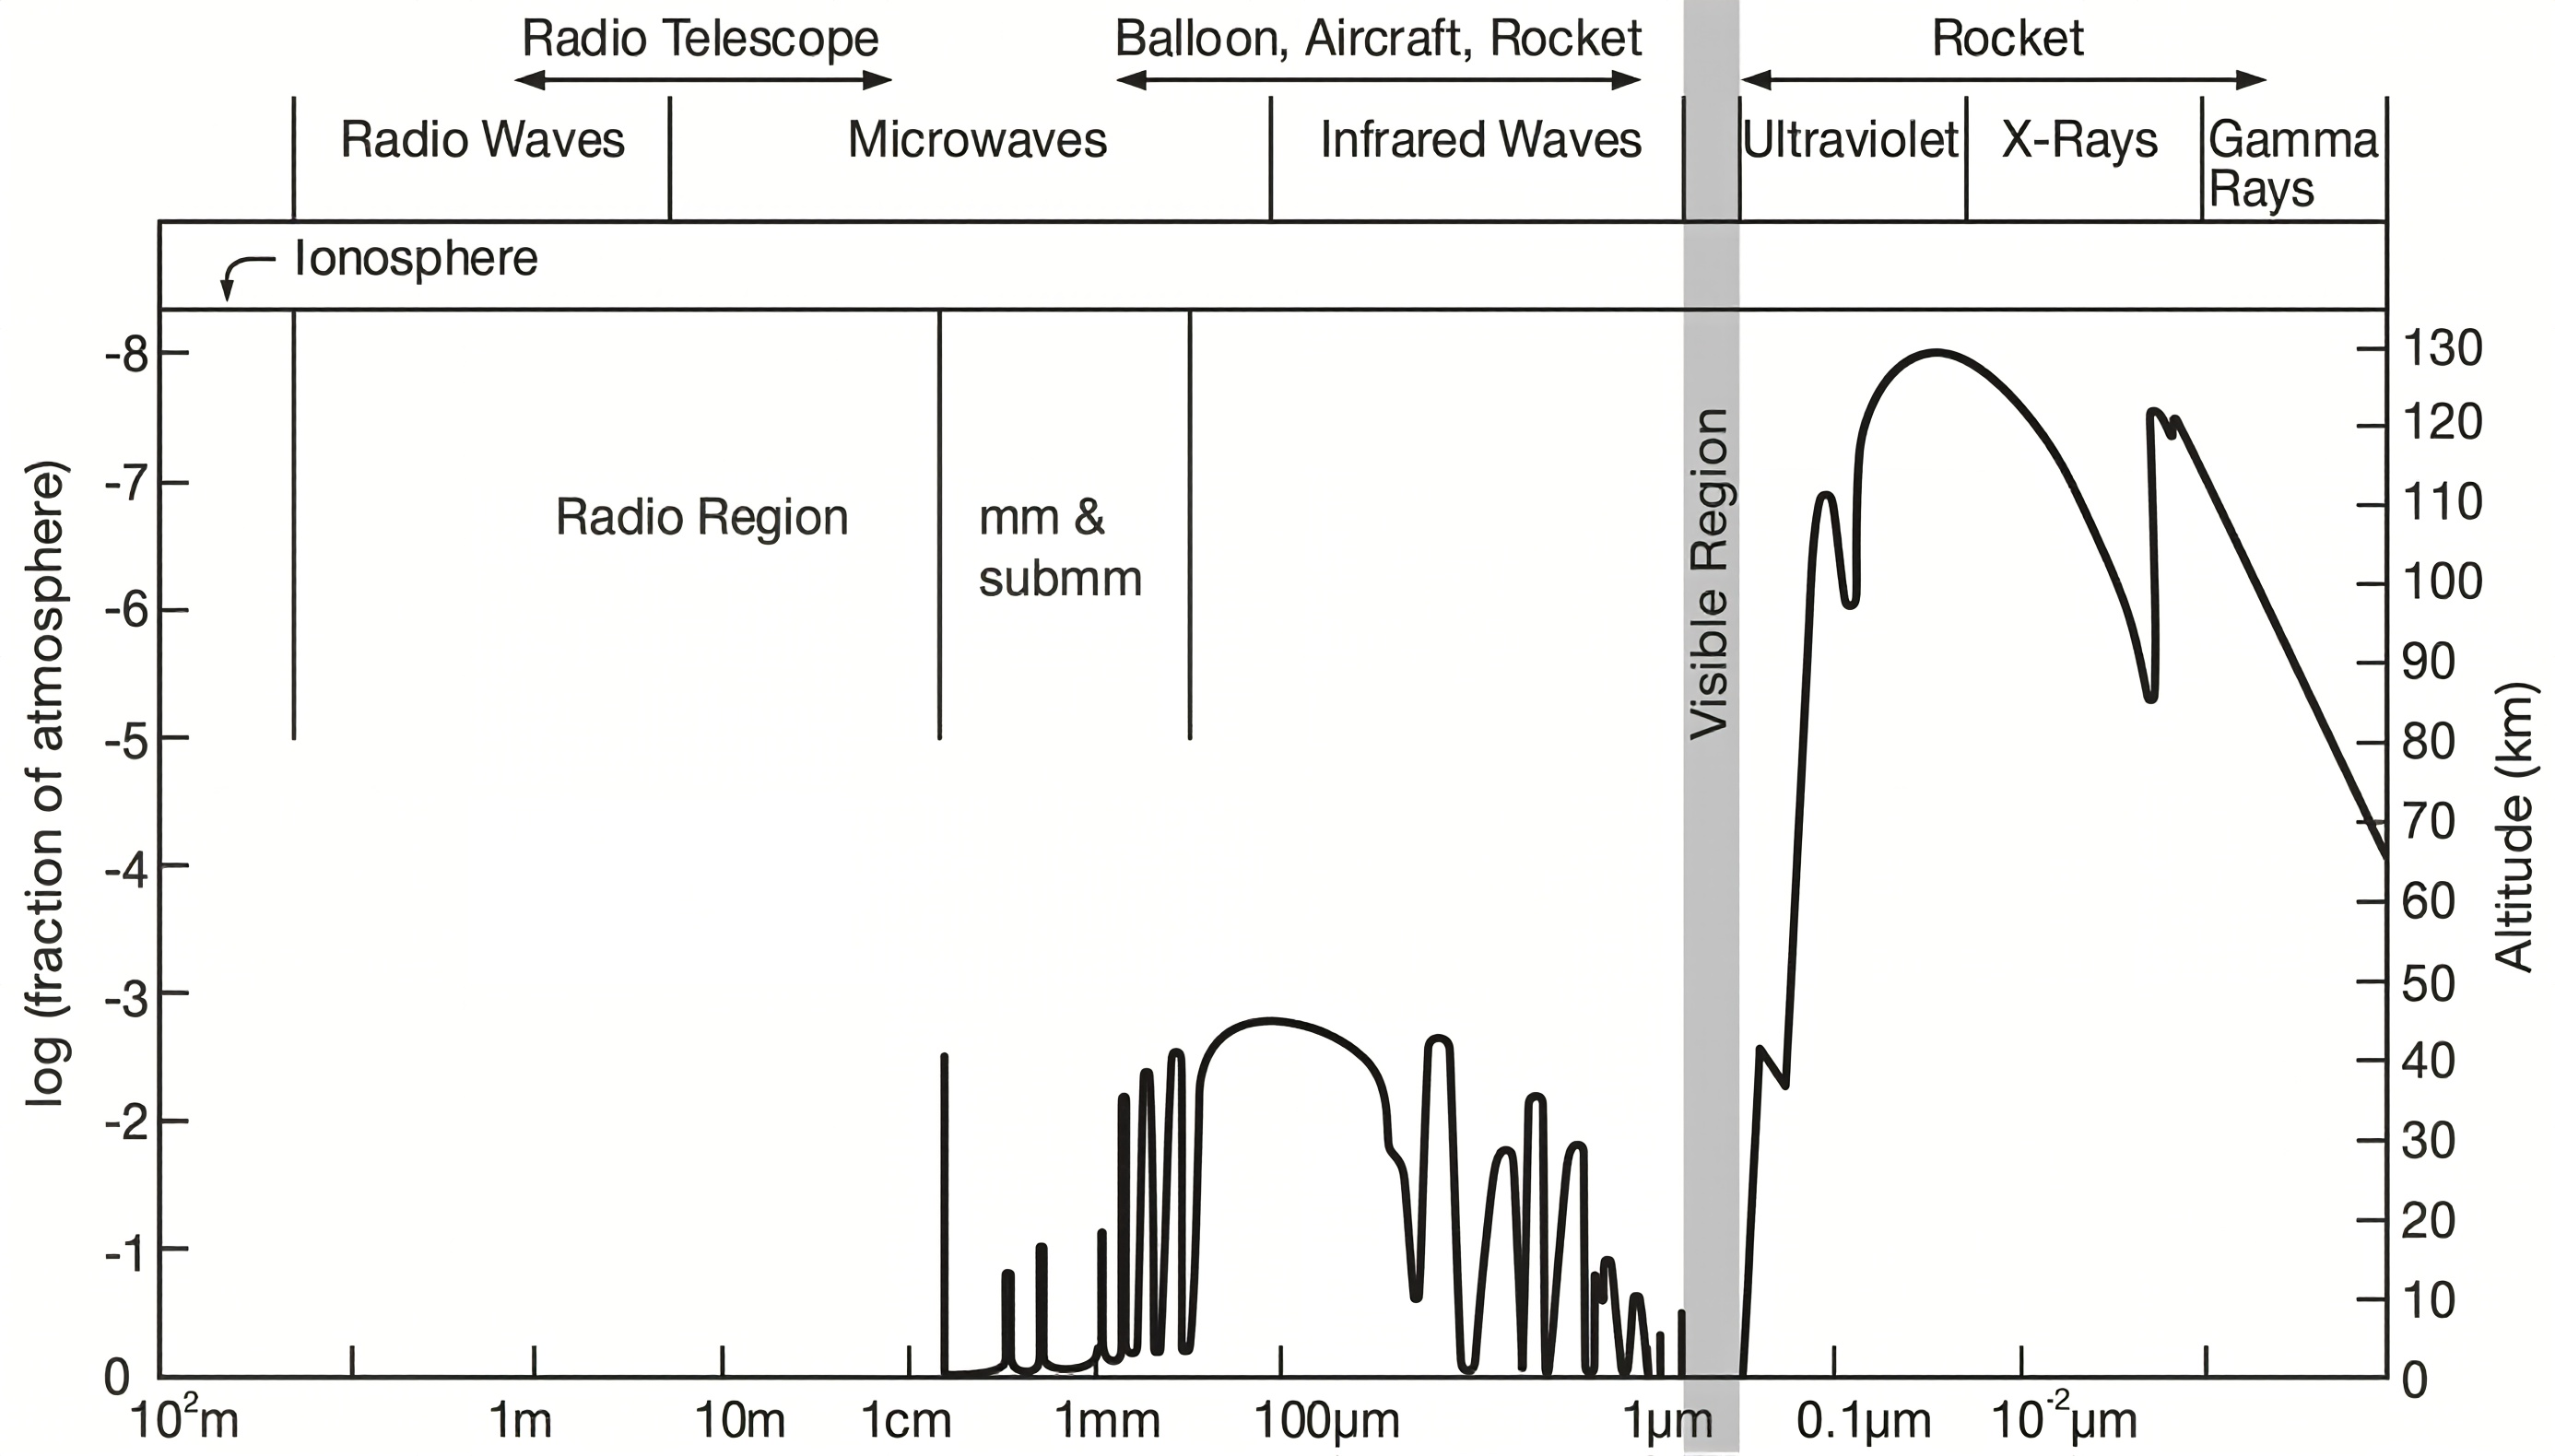
\includegraphics[width=0.55\textwidth]{assets/atmosphere_trasmission.png}
    \vspace{-0.5em}
    \caption{Atmospheric transmission as a function of wavelength.}
    \label{fig:atmosphere_transmission}
\end{figure}

\vspace{-0.8em}

Different classes of astrophysical objects emit predominantly at different wavelengths. Active galactic nuclei (AGN) are among the few source types detectable across virtually the entire electromagnetic spectrum. Other sources are more narrowly confined: galaxies, pulsars, supernova remnants (SNR), and neutral hydrogen (HI) emit strongly in the \textbf{radio}; the cosmic microwave background (CMB), dust, and molecular clouds dominate the \textbf{mm/sub-mm} bands; dust, molecular clouds, and cool K--M type stars are prominent in the \textbf{infrared}; stars, AGN, and HII regions characterise the \textbf{optical/NUV}; HII regions, stellar coronae, galaxy clusters, pulsars, X-ray binaries, AGN, and SNR populate the \textbf{UV/X-ray} regime; and the most energetic phenomena (gamma-ray bursts, AGN, pulsars) are observed in \textbf{gamma rays}.

\vspace{-0.5em}

\subsection{Information Content of Radiation} \label{subsec:information_content}

Radiation from an astronomical source carries three broad categories of physical information:

\begin{itemize}[noitemsep]
    \item \textbf{Flux}: the rate of arriving photons constrains the source \textit{luminosity}, given assumptions about its emission geometry. \textit{Periodicity} or \textit{variability} of the flux reveals it's physical nature.

    \item \textbf{Arrival direction and morphology}: whether a source is \textit{resolved} or \textit{unresolved} (limited by diffraction and atmospheric effects) determines the spatial information that can be extracted. For resolved sources, the morphology encodes the structure and physical processes at work.

    \item \textbf{Spectrum}: the photon energy distribution reveals the \textit{composition} of the source (through atomic and molecular features), its \textit{temperature} (through the continuum shape), and its line-of-sight \textit{velocity} or \textit{redshift} (through Doppler shifts of spectral features).
\end{itemize}


\section{Optical, UV, and Infrared Telescopes} \label{sec:optical_ir}

\subsection{Image Formation and Optics} \label{subsec:image_formation}

For distant astronomical sources, the incoming wavefronts can be treated as parallel rays. A lens or mirror of diameter $D$ and focal length $f$ focuses these rays to a point in the focal plane.

\begin{minipage}{0.45\textwidth}
    The optical system is characterised by two key parameters:
    \begin{itemize}
        \item \textbf{Aperture diameter}: $D$
        \item \textbf{Focal length}: $f$
    \end{itemize}
\end{minipage}%
\hfill
\begin{minipage}{0.53\textwidth}
    \centering
    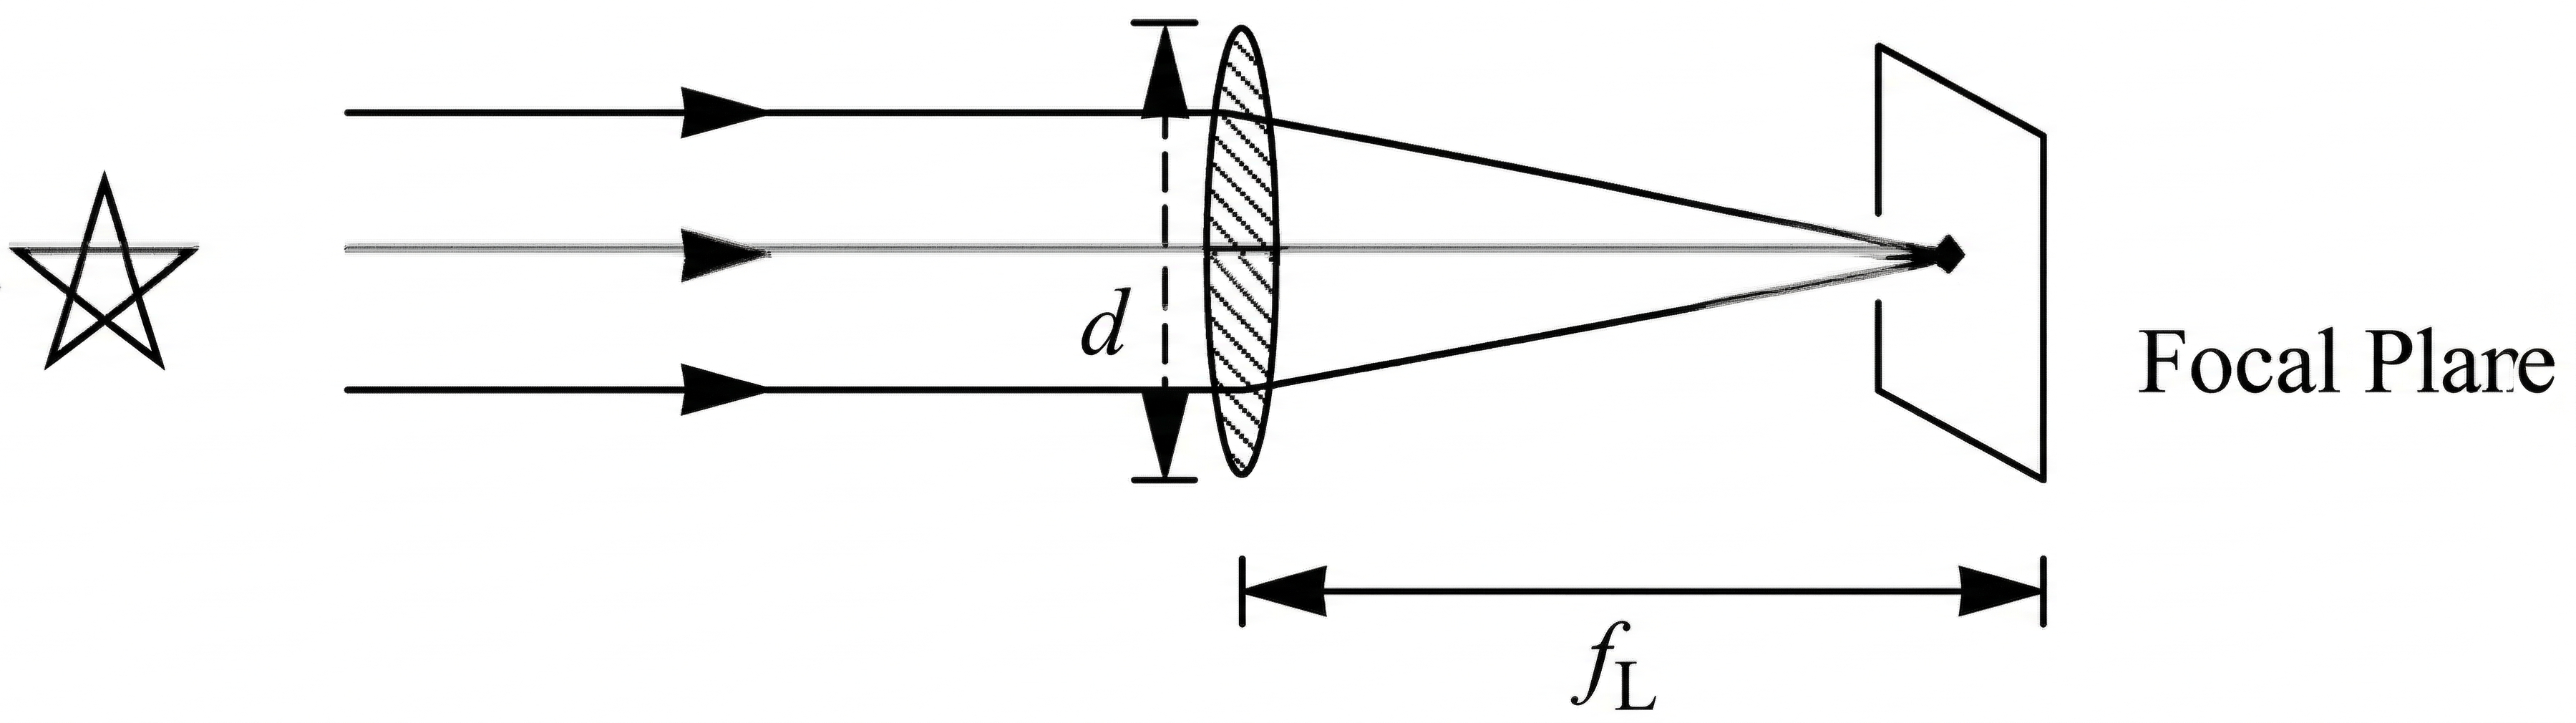
\includegraphics[width=\textwidth]{assets/image_formation.png}
    % \captionof{figure}{Image formation}
\end{minipage}

\medskip

The \bfit{focal ratio} $R$ is defined as the ratio of the focal length to the aperture diameter:

$$
R = \dfrac{f}{D}
$$

The focal ratio governs the irradiance (power per unit area) delivered to the focal plane, which scales as $E_p \propto 1/R^2$. Systems with a low focal ratio ($R \sim 4$--$5$), termed \textbf{fast} optical systems, concentrate light onto a small detector area and are therefore well suited for detecting extended, low surface brightness objects. Conversely, \textbf{slow} optical systems ($R \sim 10$--$15$) provide higher angular magnification and are more appropriate for point-source photometry and high-resolution imaging.

\medskip

\begin{minipage}{0.5\textwidth}

The position of the focal point in the focal plane depends on the angle $\alpha$ of the incoming light relative to the optical axis:
$$
s = f \tan \alpha \approx f\,\alpha
$$

The \bfit{plate scale}, which relates angular displacement on the sky to physical displacement in the focal plane, is therefore:

\end{minipage}
\hfill
\begin{minipage}{0.48\textwidth}
    \centering
    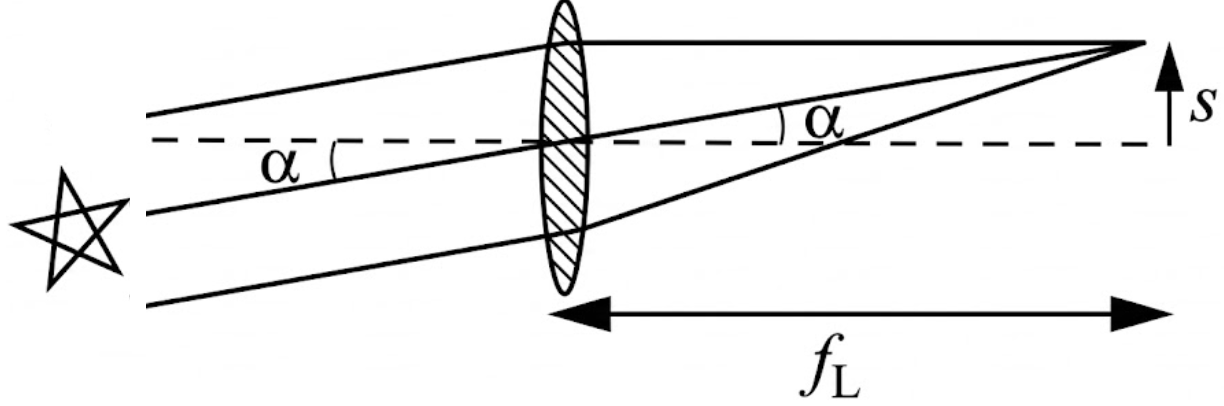
\includegraphics[width=\textwidth]{assets/image_formation_2.png}
    % \captionof{figure}{Focal point variation}
\end{minipage}
 
$$
\text{PS} = \dfrac{\alpha}{s} = \dfrac{1}{f}
$$

The \textbf{field of view} (FoV) is determined by both the focal length and the physical size $d_{\text{det}}$ of the detector in the focal plane:

$$
\text{FoV} = 2 \arctan \left( \dfrac{d_{\text{det}}/2}{f} \right) \approx \dfrac{d_{\text{det}}}{f} = d_{\text{det}} \cdot \text{PS}
$$

\begin{table}[h]
    \centering
    \small
    \renewcommand{\arraystretch}{1.3}
    \begin{tabular}{@{} l c c @{}}
        \toprule
        \textbf{Characteristic} & \textbf{James Webb (JWST)} & \textbf{Euclid} \\
        \midrule
        Mirror Diameter & 6.5\,m & 1.2\,m \\
        Focal Length & $\sim$131\,m & 24.5\,m \\
        Focal Ratio & 20 & 20 \\
        Field of View & Very narrow: $\sim$arcmin (depth) & Very wide: 0.57\,deg$^2$ (survey) \\
        Cosmological Objective & First stars and galaxies & Dark matter/energy (statistics) \\
        \bottomrule
    \end{tabular}
    \caption{Comparison between JWST and Euclid.}
    \label{tab:jwst-euclid-comparison}
\end{table}

\begin{observationblock}[FoV and focal ratio]
Although JWST and Euclid share the same focal ratio ($R = 20$), their fields of view differ dramatically. This apparent paradox is resolved by recognising that the FoV depends on the \textbf{detector size}, not just the focal ratio. Euclid achieves its wide field of view by employing a large mosaic of detectors at its focal plane, effectively increasing the physical dimension $d_{\text{det}}$ of the detection area. Since $\text{FoV} \approx d_{\text{det}}/f$, a larger detector array directly translates to a wider field of view, even when the focal ratio remains constant.
\end{observationblock}


\subsection{Telescope Configurations} \label{subsec:telescope_configs}

Two fundamental telescope designs exist, distinguished by how they focus incoming light.

\begin{itemize}
    \item \textbf{Refractor telescopes} 
    
    use lenses as their primary optical element. Aberrations can be greatly reduced (or effectively eliminated) through aspherical, achromatic, and multi-element lens systems at both the objective and the eyepiece. However, refractors suffer from several intrinsic limitations: large lenses are heavy and deform under their own weight; chromatic aberration cannot be fully eliminated; light is partially absorbed within the glass; and achieving long focal lengths requires physically long telescope tubes with correspondingly massive support structures and large domes. The largest refractor ever built for astronomical use is the 1.02\,m (40-inch) Yerkes Observatory telescope, established by the University of Chicago in 1897.
    
    \item \textbf{Reflector telescopes} 
    
    use mirrors as their primary optical element and dominate modern observational astronomy. Mirrors can be supported from the back, allowing gravitational deformations to be corrected using active optics; they introduce no chromatic aberration; they can achieve higher reflectivity than lenses achieve in transparency; and, by folding the optical path through multiple reflections inside the telescope tube, the overall structure can be made shorter for a given focal length, reducing the size and cost of the dome and support structure.
\end{itemize}

\begin{figure}[H]
    \centering
    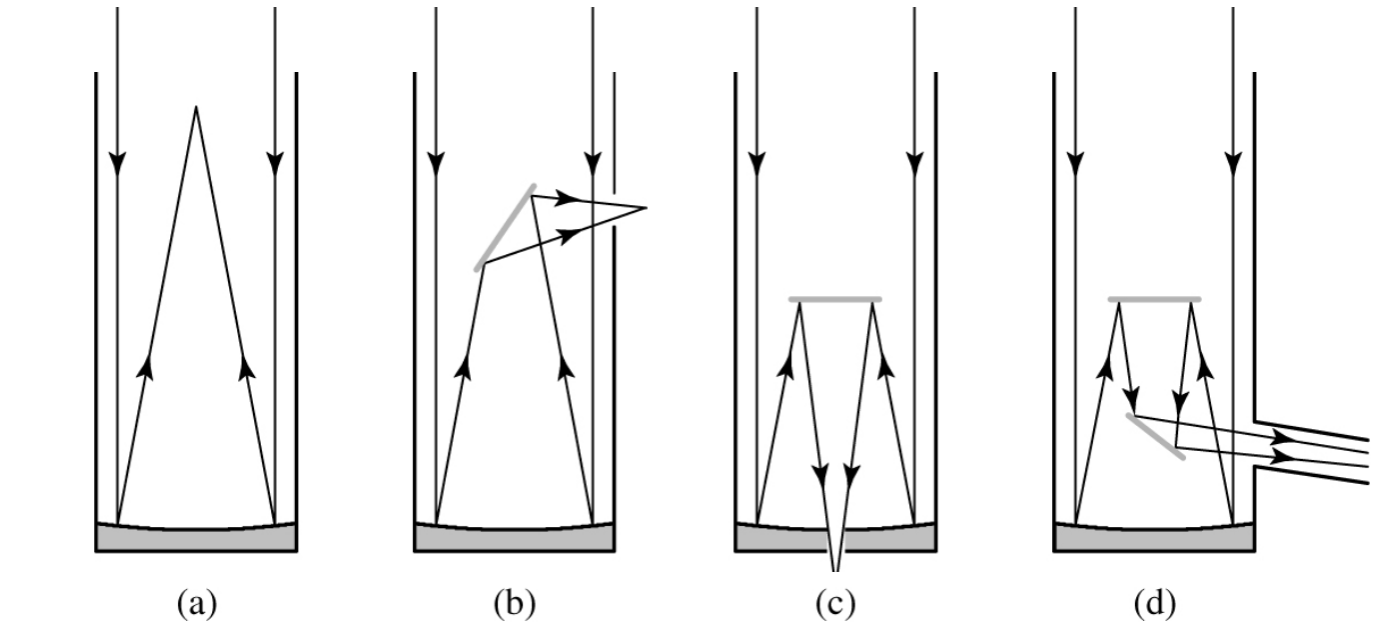
\includegraphics[width=0.75\textwidth]{assets/reflectors_config.png}
    \caption{(a) prime focus, (b) Newtonian, (c) Cassegrain, (d) Nasmyth/Coudé.}
    \label{fig:reflectors_configurations}
\end{figure}

Several focal configurations are available for reflectors (\cref{fig:reflectors_configurations}). Wide-field cameras are typically deployed at the \textbf{prime focus} to take advantage of the shortest possible focal length. If the secondary mirror is curved rather than flat (e.g. \textbf{Newtonian} or \textbf{Cassegrain} configurations), the effective focal length of the system can be modified. The \textbf{Coudé} (or \textbf{Nasmyth}) configuration uses an additional flat mirror to transport the beam to a fixed location, typically a very stable spectrograph with a controlled temperature; this comes at the cost of a longer effective focal length.


\subsection{Detectors} \label{subsec:detectors}

\subsubsection{Photographic Plates}

For over a century, photographic plates served as the primary detector in astronomy. These devices consist of a glass substrate coated with a light-sensitive emulsion: when a photon is absorbed, it triggers a chemical change in the emulsion, and subsequent chemical development produces a permanent image. A key limitation is their \textbf{non-linear response}: as the plate is exposed, the density of unreacted light-sensitive molecules decreases, so the probability of detecting additional photons drops and sensitivity falls off at high illumination levels.

\subsubsection{CCD Detectors}

A \bfit{Charge Coupled Device} (CCD) is a two-dimensional array of silicon pixels that converts incoming photons into stored electric charge. Each pixel acts as a potential well in which photo-electrons accumulate during the exposure. CCD surfaces are typically divided into $2048$ to $4096$ pixels per side, with a characteristic pixel size of ${\sim}\,10\;\mu$m, corresponding to a total chip size of ${\sim}\,2.5$\,cm. High linearity and broad wavelength sensitivity have made CCDs the most suited detector for optical astronomy, and modern large-area survey cameras are built from mosaics of many CCD chips.

\begin{figure}[H]
    \centering
    \begin{minipage}{0.55\textwidth}
        \centering
        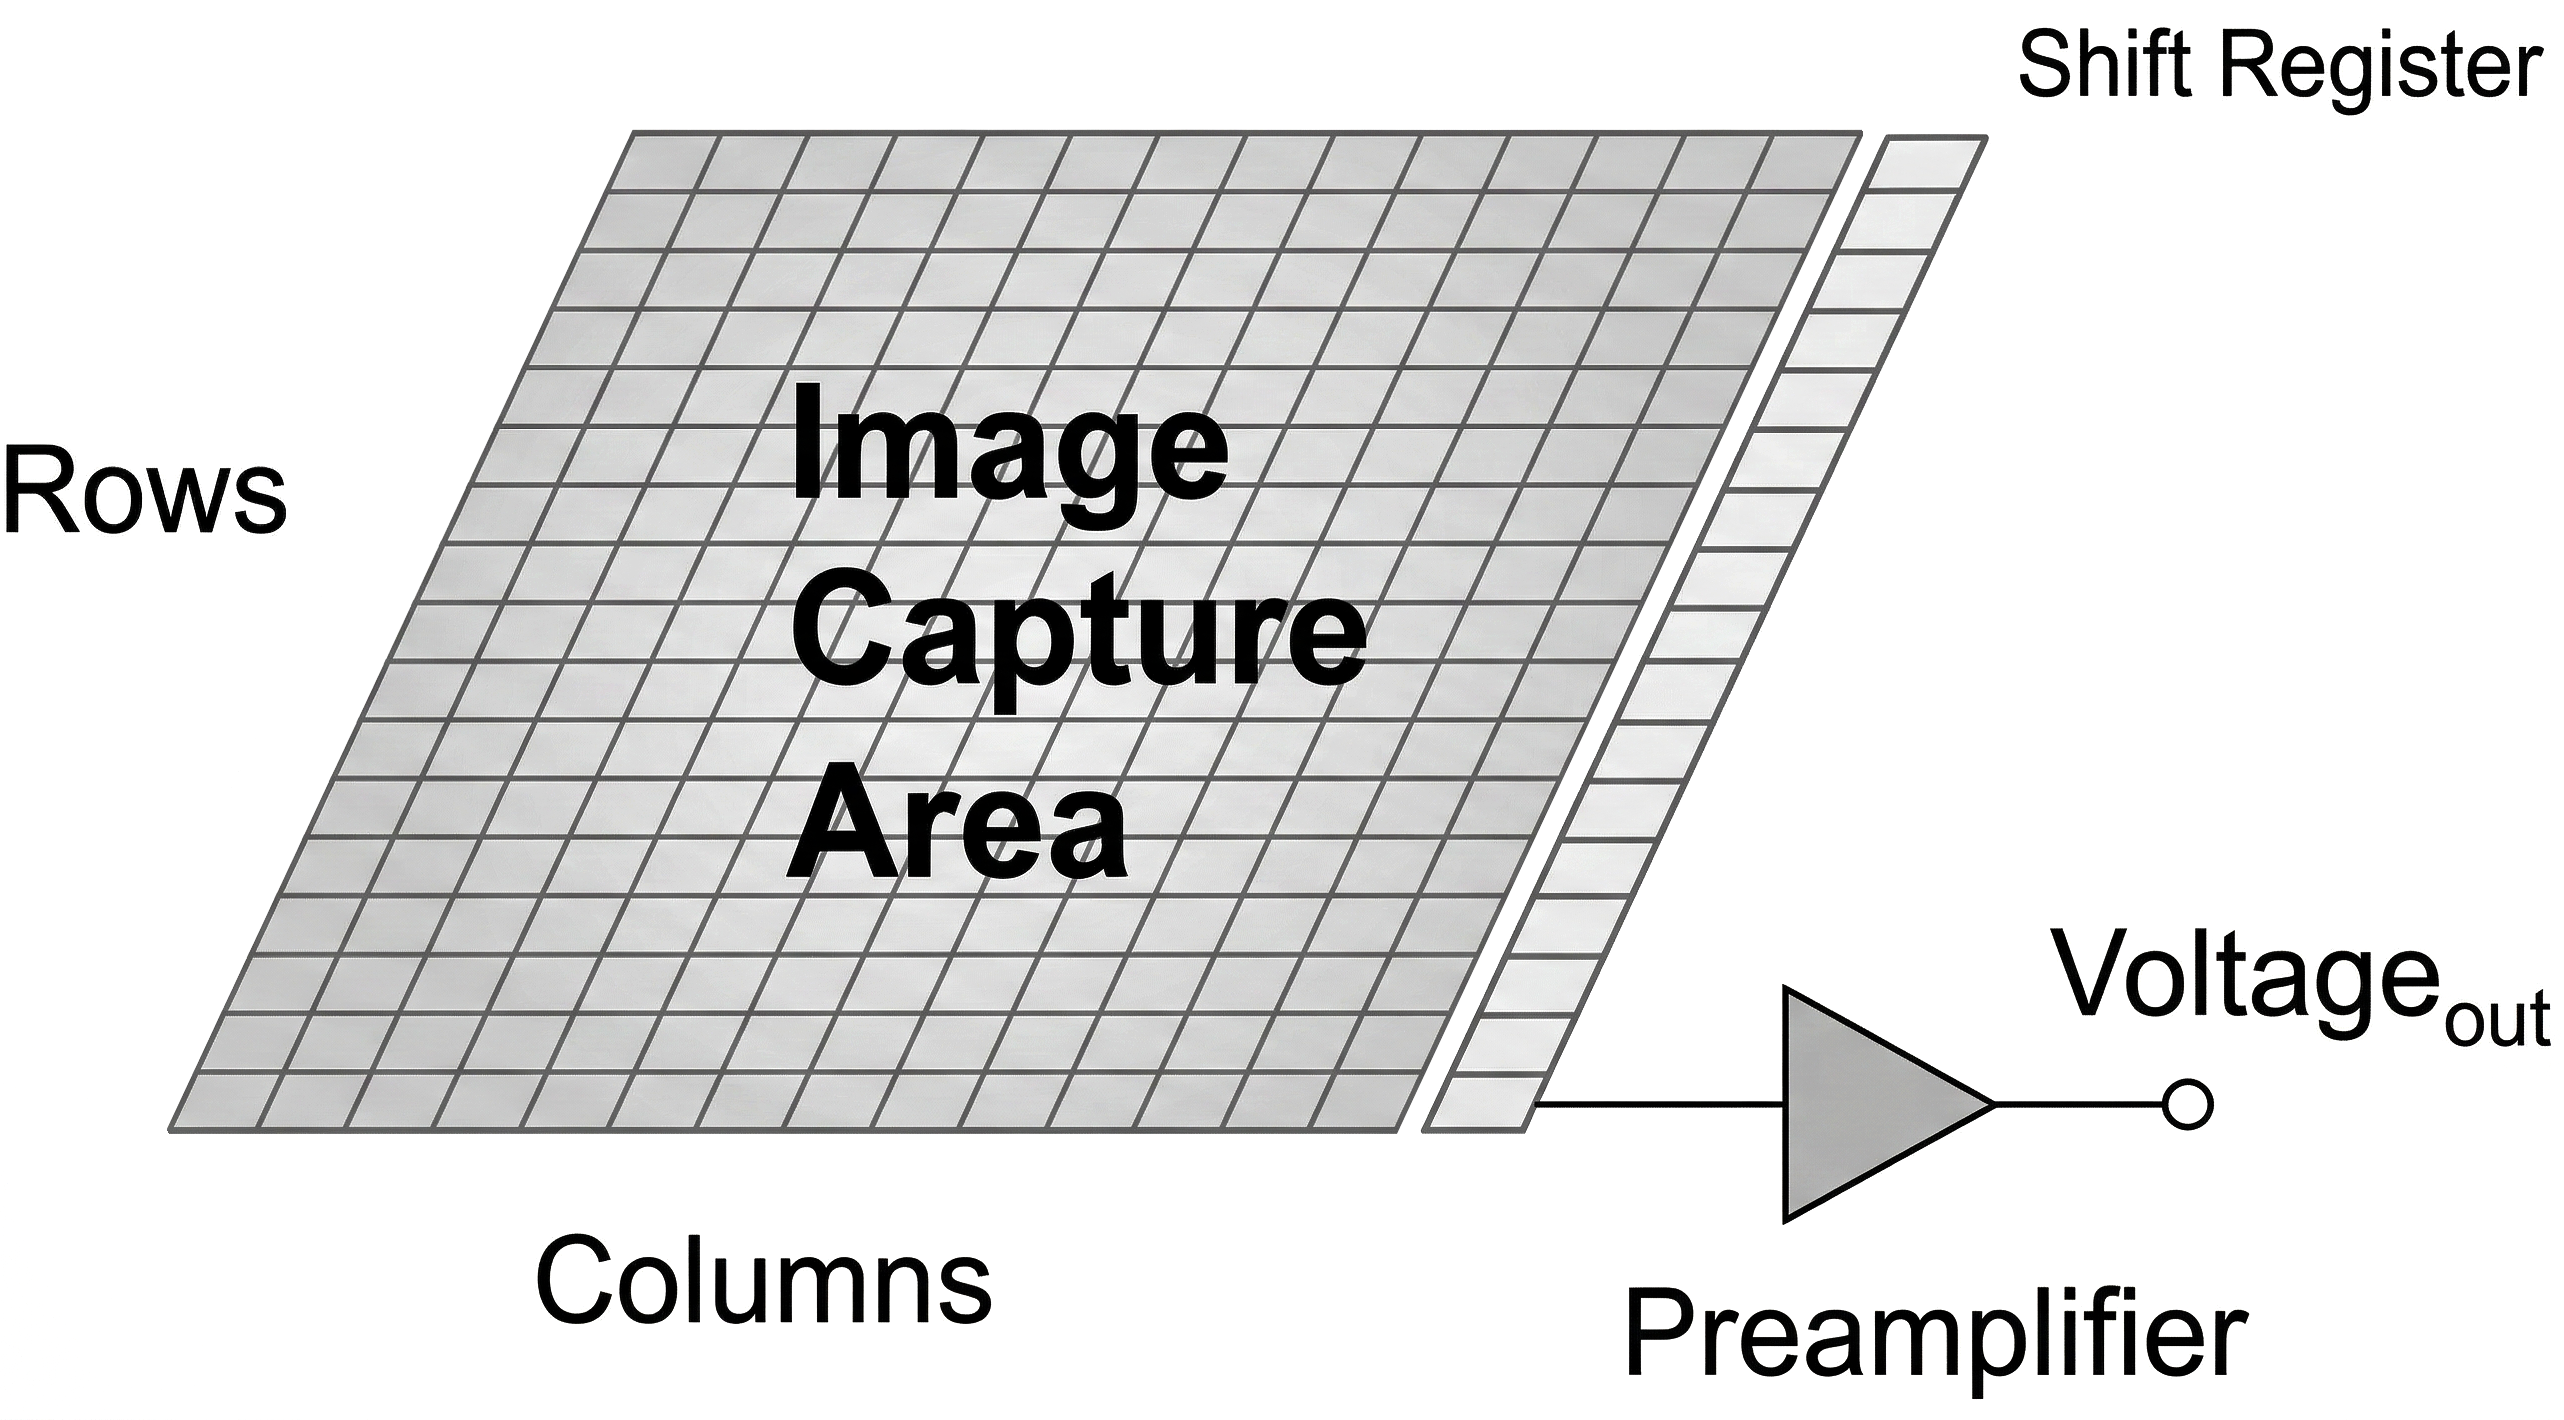
\includegraphics[width=0.8\textwidth]{assets/ccd.png}
        \captionof{figure}{\textbf{Left}: Schematic of a CCD. \textbf{Right}: Rain bucket analogy: photons (rain) fall into pixel wells arranged in vertical columns; during readout, accumulated charge is shifted row by row into a horizontal serial register, then measured at the output node.}
    \end{minipage}
    \hfill
    \begin{minipage}{0.43\textwidth}
        \centering
        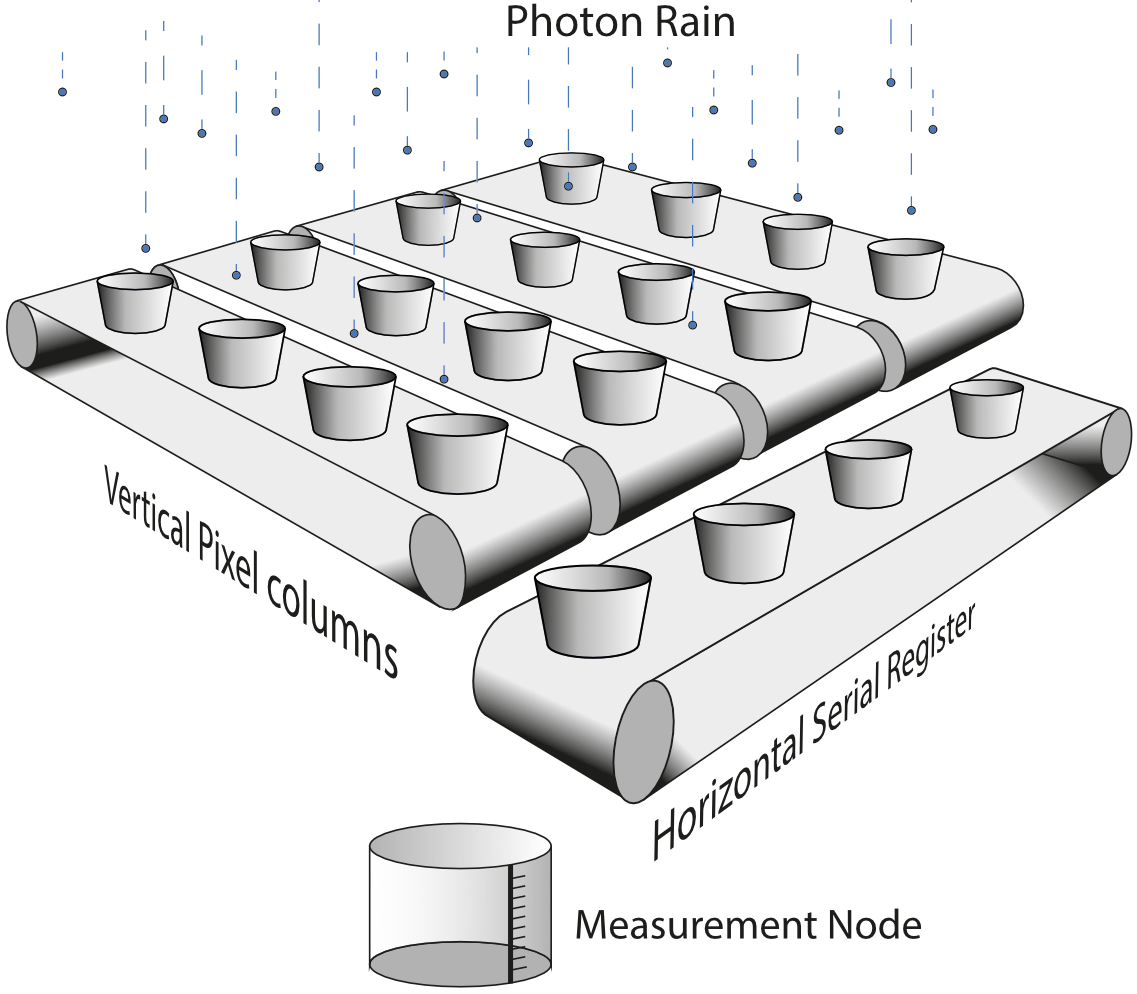
\includegraphics[width=\textwidth]{assets/ccd_analogy.png}
    \end{minipage}
    \label{fig:ccd_analogy}
\end{figure}

The key performance characteristics of CCDs are:

\begin{itemize}
    \item \textbf{High quantum efficiency}: the ratio $\text{QE} = N_{e^-\!} / N_\gamma$ of collected electrons to incoming photons reaches 80\% or higher, compared to ${\sim}\,1\%$ for the human eye or photographic plates.
    \item \textbf{Broad spectral sensitivity}: CCDs respond to all photons with energy above the silicon band gap ($E > 1.11$\,eV, or equivalently $\lambda < 1.1\;\mu$m).
    \item \textbf{High dynamic range}: the linear response spans a dynamic range of ${\sim}\,10^5$, from a read-noise floor of 1--2\,$e^-$ to a full-well capacity of ${\sim}\,10^5\;e^-$ (compared to ${\sim}\,10^2$ for photographic plates).
\end{itemize}

These properties have enabled quantitative photometric measurements of extended sources, time-domain astronomy, and the large wide-field surveys (e.g.\ Sloan Digital Sky Survey, Pan-STARRS, Dark Energy Survey, Euclid, LSST) that have transformed modern cosmology.

\begin{minipage}{0.72\textwidth}
    Raw CCD images typically contain unwanted instrumental signatures: readout amplifiers may introduce different bias levels, bright sources can cause saturation or charge bleeding along columns, and electronic defects manifest as dead or hot pixels. 
    
    Additional contamination arises from cosmic-ray hits, scattered light, and satellite trails. Single-epoch images must therefore be \textbf{calibrated} to remove these artefacts before scientific analysis. \textbf{Coadded images}, which combine multiple calibrated single-epoch exposures, represent the final science-ready data products.
\end{minipage}%
\hfill
\begin{minipage}{0.25\textwidth}
    \centering
    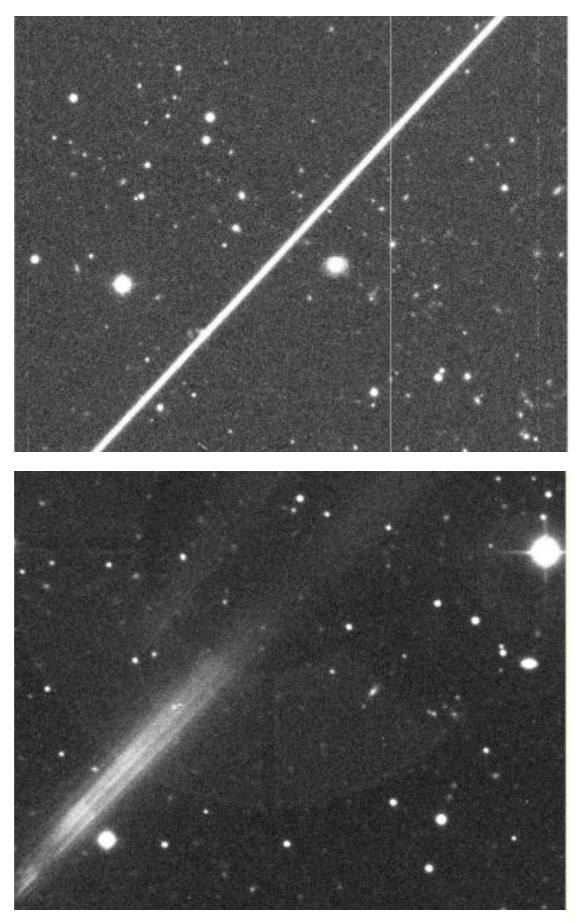
\includegraphics[width=0.95\textwidth]{assets/ccd_artifacts.png}
\end{minipage}

\vspace{-2em}

\subsubsection{CMOS Detectors}

The silicon band gap renders standard CCDs insensitive to photons with wavelengths beyond ${\sim}\,1\;\mu$m. For infrared observations, hybrid \bfit{Complementary Metal-Oxide-Semiconductor} (CMOS) detectors are used instead. In a CMOS detector, each pixel contains its own readout electronics (a charge-to-voltage converter and amplifier), so charge is converted to a voltage signal locally rather than being shifted across the entire array as in a CCD. This architecture eliminates charge-transfer losses and enables high readout speeds.

CMOS detectors for astronomy couple a photodiode layer made from a material photosensitive at the desired infrared wavelength (typically HgCdTe, mercury cadmium telluride) to a silicon readout circuit, forming a \textbf{hybrid device}. By adjusting the cadmium fraction $x$ in Hg$_{1-x}$Cd$_x$Te, the band gap (and hence the wavelength sensitivity) of the detector can be tuned (\cref{fig:cmos_hgcdte}). Sensitivity to low-energy infrared photons requires cryogenic operating temperatures ($T < 100$\,K) to suppress thermal noise (dark current).

\begin{figure}[H]
    \begin{minipage}{0.4\textwidth}
        \centering
        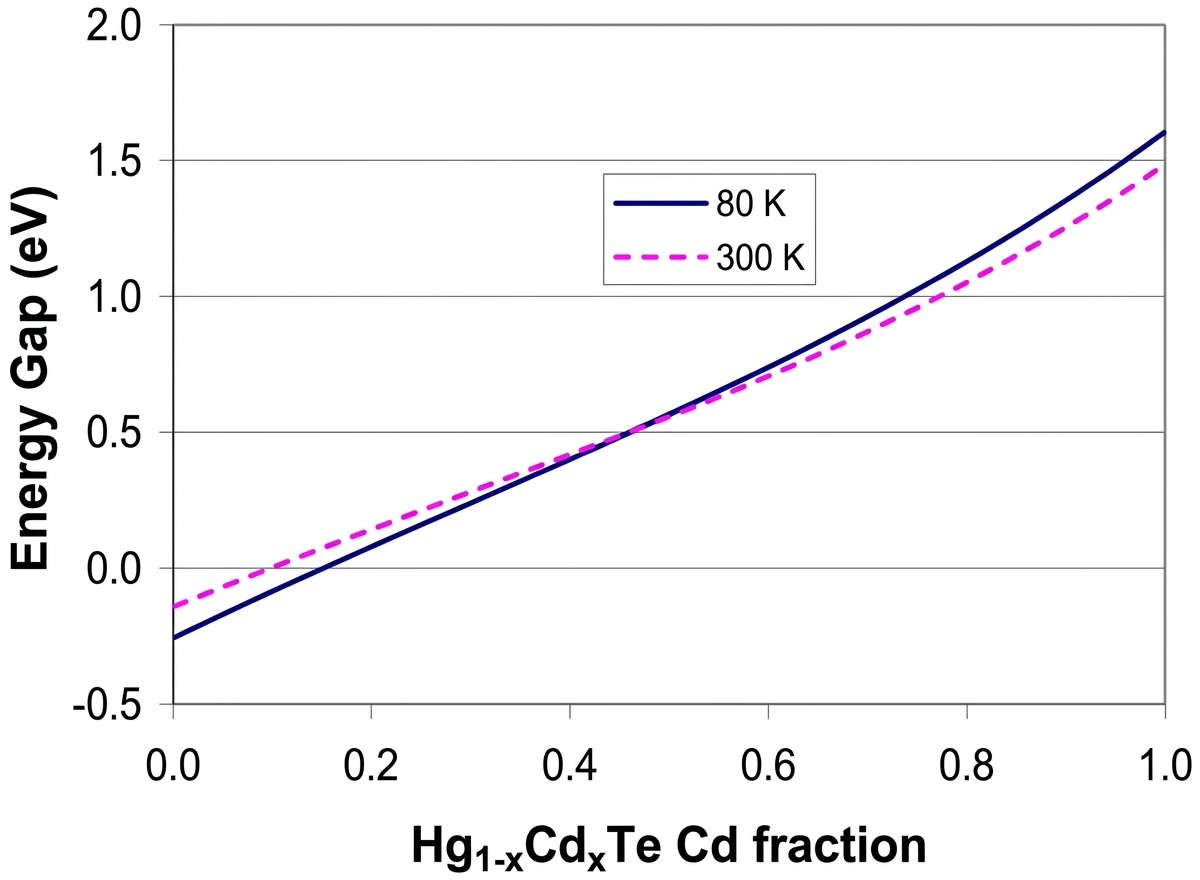
\includegraphics[width=\textwidth]{assets/cmos.png}
    \end{minipage}%
    \hfill
    \begin{minipage}{0.55\textwidth}
        \caption{HgTe is a semimetal and CdTe is a semiconductor. By adjusting the Cd fraction, the wavelength sensitivity of HgCdTe arrays can be tuned. The plot shows the energy gap as a function of Hg$_{1-x}$Cd$_x$Te Cd fraction at several temperatures.}
        \label{fig:cmos_hgcdte}
    \end{minipage}
\end{figure}

\begin{minipage}{0.72\textwidth}
    Ground-based infrared images are typically background-limited: the sky is so bright in the IR that individual exposures must be kept very short (${\sim}\,10$\,s). Observations are further complicated by the narrow atmospheric transmission windows in the $J$, $H$, and $K$ bands, caused by strong molecular absorption from H$_2$O, CO$_2$, and CH$_4$. 
    
    To build up signal, large series of short exposures are taken with small spatial offsets (dithers); the sky background is subtracted and the individual frames are coadded, analogously to the optical CCD pipeline.

    \medskip

    From space, the infrared background is much lower (dominated by zodiacal light), although the particle background from cosmic rays is correspondingly higher.
\end{minipage}%
\hfill
\begin{minipage}{0.25\textwidth}
    \centering
    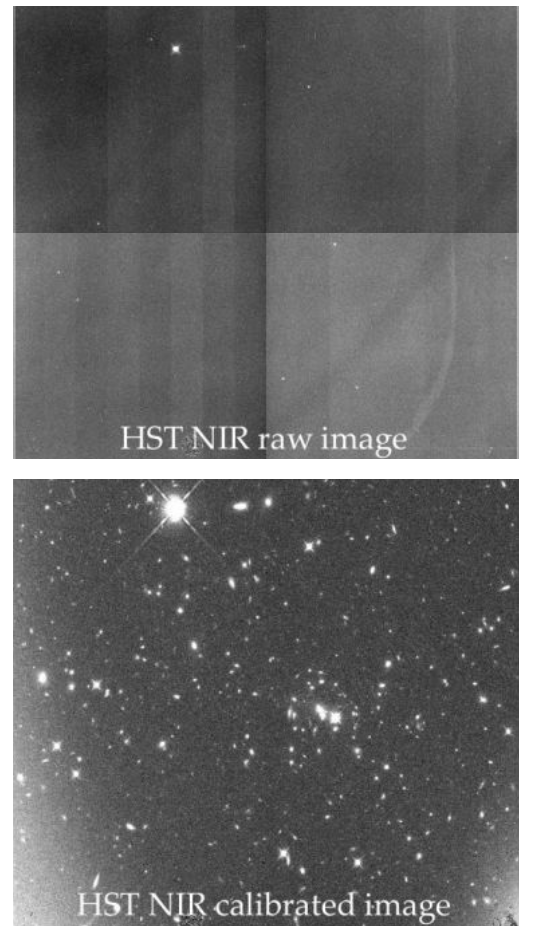
\includegraphics[width=0.9\textwidth]{assets/cmos_artifacts.png}
\end{minipage}

\subsubsection{Photometric Passbands}

In optical and NIR photometry, measurements are performed through standardised filters that transmit light within defined wavelength intervals. The standard broadband filters are listed in \cref{fig:pau_bands}. Narrow-band filters are also widely used to isolate specific spectral lines or features, and to improve constraints on the spectral energy distribution of a source. An example is the PAU camera, which employs 40 narrow-band filters to provide finely sampled photometric redshifts.

\begin{figure}[H]
    \centering
    \begin{minipage}{0.45\textwidth}
        \centering
        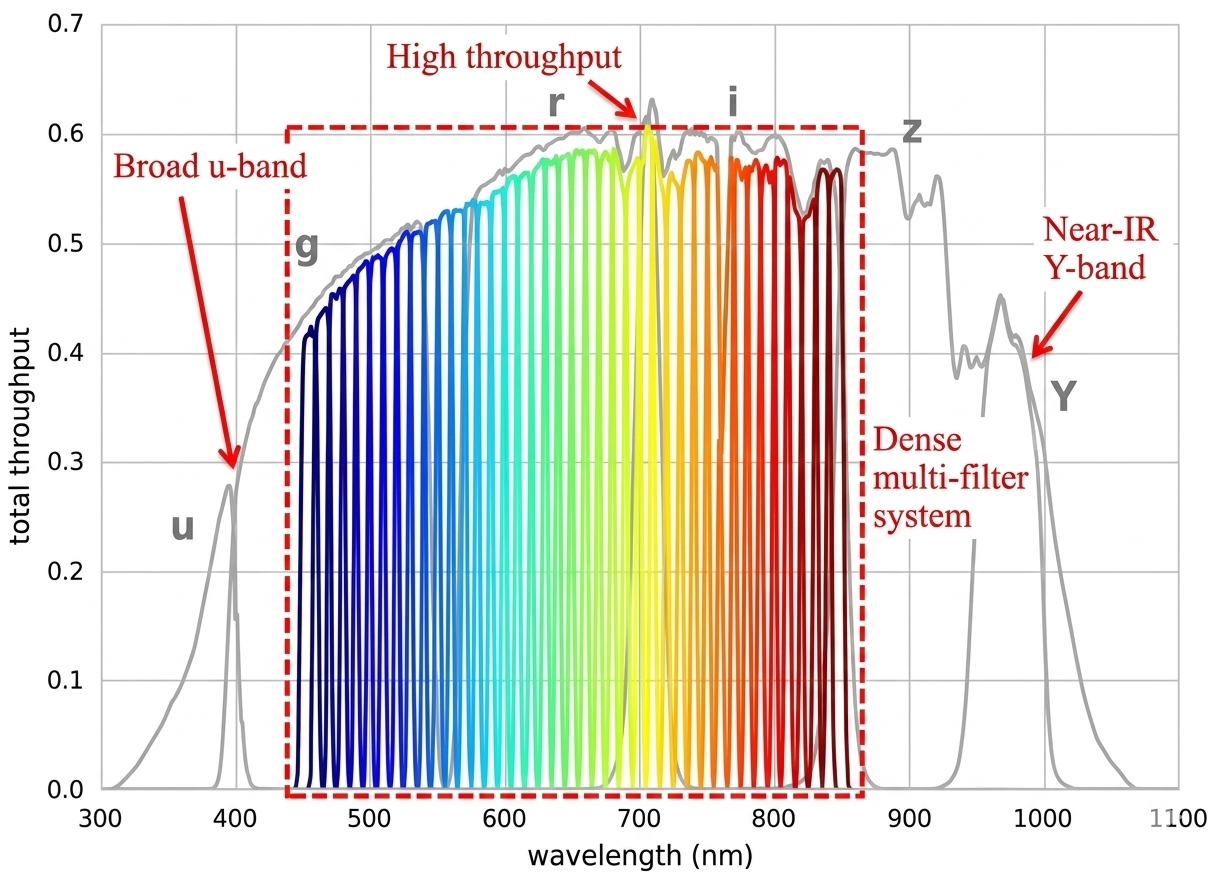
\includegraphics[width=\textwidth]{assets/pau_bands.png}
        \caption{Narrow bands of PAU camera.}
        \label{fig:pau_bands}
    \end{minipage}%
    \hspace{2em}
    \begin{minipage}{0.4\textwidth}
        \centering
        \small
        \begin{tabular}{c c c}
            \toprule
            \textbf{Band} & $\lambda_{\text{mid}}$ [nm] & $\Delta\lambda$ [nm] \\
            \midrule
            U & 365 & 66 \\
            B & 445 & 94 \\
            V & 551 & 88 \\
            R & 658 & 138 \\
            I & 806 & 149 \\
            Z & 900 & \\
            Y & 1020 & 120 \\
            J & 1220 & 213 \\
            H & 1630 & 307 \\
            K & 2190 & 390 \\
            L & 3450 & 472 \\
            M & 4750 & 460 \\
            \bottomrule
        \end{tabular}
    \end{minipage}
\end{figure}


\subsection{Angular Resolution: Ground versus Space} \label{subsec:angular_resolution}

For space-based telescopes (or small ground-based telescopes), the angular resolution is limited by diffraction at the telescope aperture. The diffraction pattern produced by a circular aperture is called the \bfit{Airy pattern}: a bright central disc containing 83.3\% of the total energy, surrounded by progressively fainter concentric rings. The angular radius of the first minimum, which defines the \textbf{Airy disc}, is  $\theta = 1.22\,\frac{\lambda}{D}$, where $\lambda$ is the observing wavelength and $D$ is the aperture diameter.

\begin{figure}[H]
    \centering
    \begin{minipage}{0.45\textwidth}
        \centering
        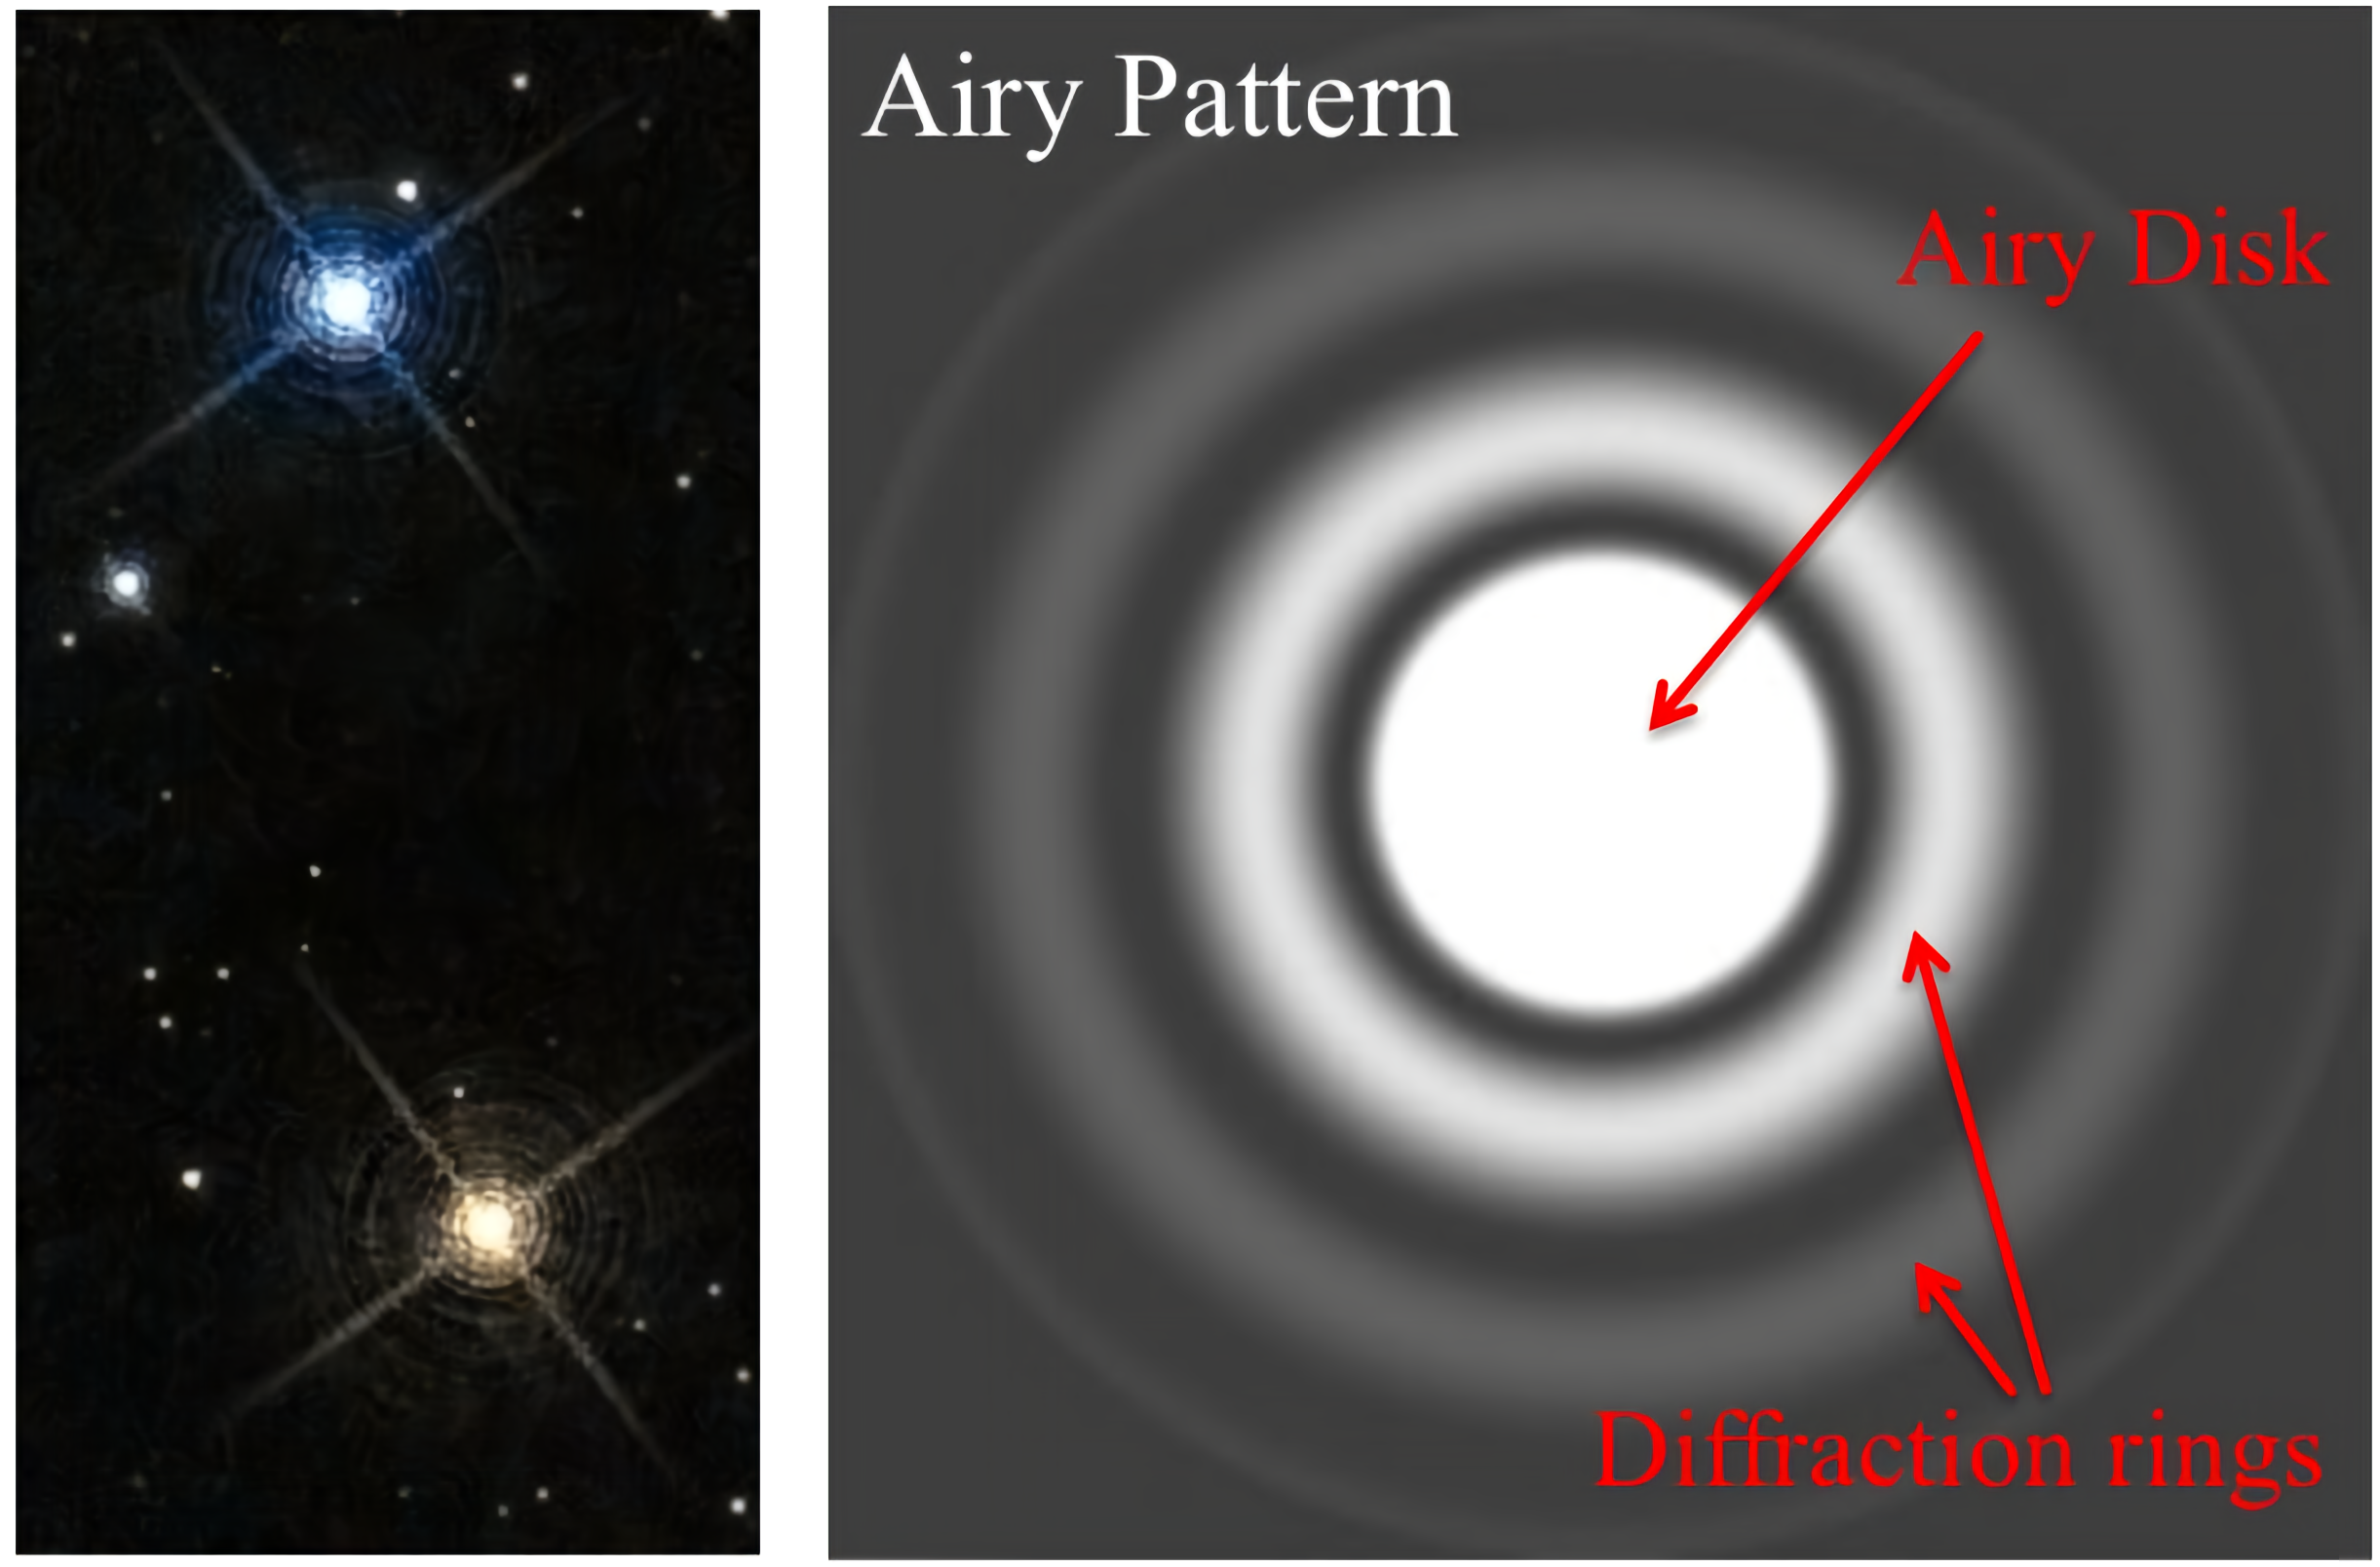
\includegraphics[width=0.95\textwidth]{assets/airy_effect.png}
    \end{minipage}%
    \hfill
    \begin{minipage}{0.53\textwidth}
        \centering
        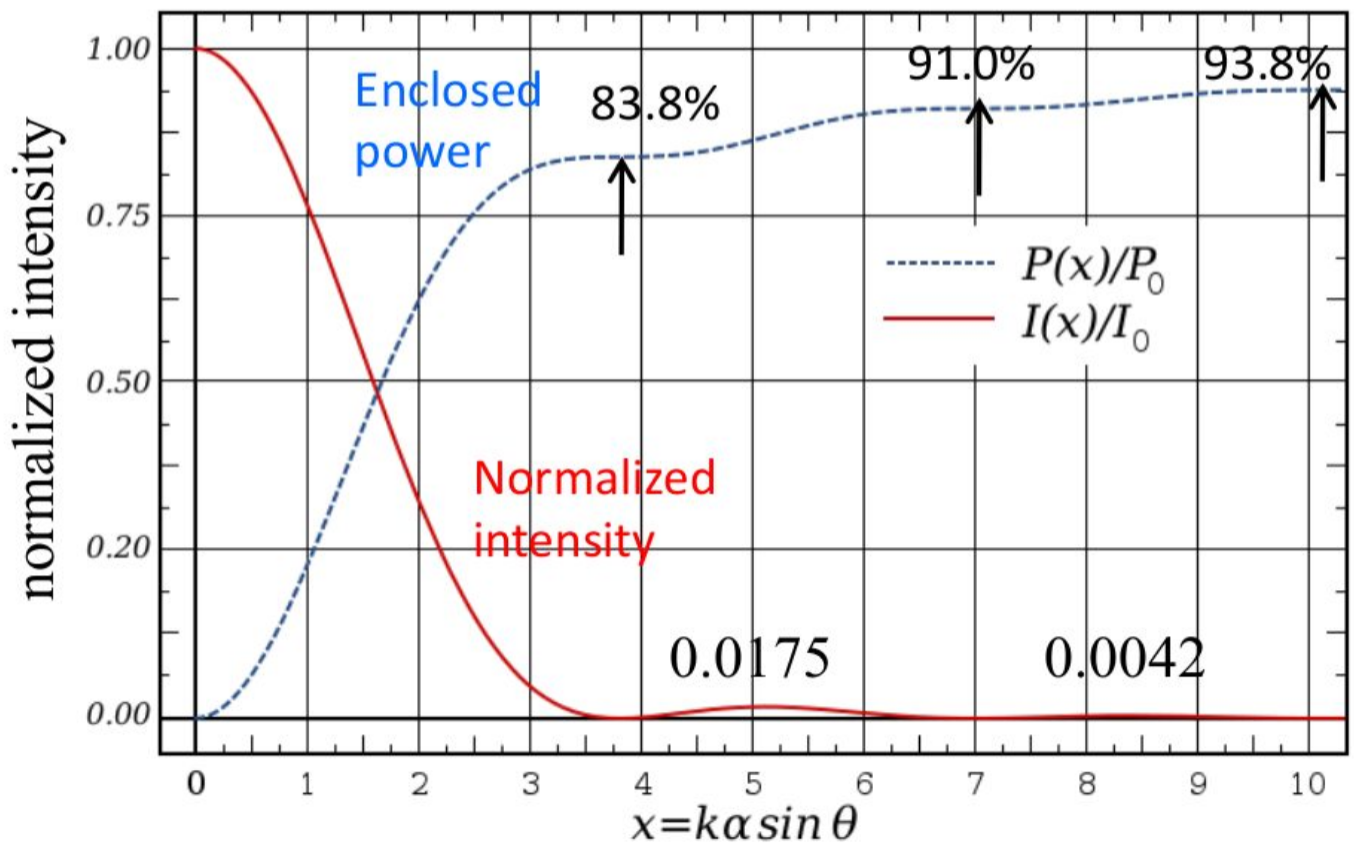
\includegraphics[width=0.95\textwidth]{assets/intensity.png}
    \end{minipage}
    \caption{The Airy diffraction pattern (left) and its radial intensity profile (right).}
    \label{fig:airy_effect}
\end{figure}

\subsubsection{Rayleigh Criterion}

The \bfit{Rayleigh criterion} states that two point sources are just resolved when the central maximum of one coincides with the first minimum of the other, requiring an angular separation:

$$
\Delta\theta > 1.22\,\frac{\lambda}{D}
$$

This criterion corresponds closely to the full-width at half-maximum (FWHM) of the Airy disc, which provides a more convenient operational measure of the angular resolution. 

\begin{observationblock}[Diffraction-limited resolution]
At $\lambda = 0.5\;\mu$m), the diffraction-limited resolution of some representative telescopes is:

\begin{itemize}
    \item 2.4\,m Hubble Space Telescope: $\theta_{\min} \approx 0.05''$
    \item 4\,m (e.g.\ Canada-France-Hawaii Telescope): $\theta_{\min} \approx 0.03''$
    \item 8.2\,m Subaru Telescope: $\theta_{\min} \approx 0.015''$
\end{itemize}

For comparison, the angular resolution of the human eye at night is approximately $20''$.
\end{observationblock}

\begin{minipage}{0.57\textwidth}
For large ground-based telescopes, however, the point-spread function (PSF) is dominated by atmospheric turbulence rather than telescope optics. The resulting PSF is well described by a \textbf{Moffat profile}:

$$
I(r) = \frac{I_0}{\bigl(1 + r^2/R^2\bigr)^\beta} + B
$$

where $R$ parameterises the width, $\beta$ the wing shape, and $B$ the background level. 
\end{minipage}%
\hfill
\begin{minipage}{0.4\textwidth}
    \centering
    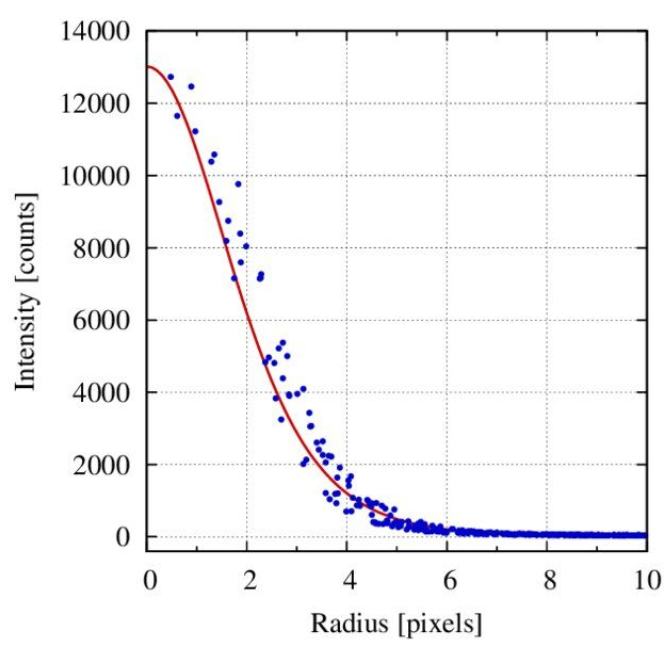
\includegraphics[width=0.9\textwidth]{assets/moffat.png}
\end{minipage}

The \bfit{seeing disc}, defined as the FWHM of the atmospheric PSF, sets the effective resolution of ground-based observations. A seeing of $0.5''$ represents excellent conditions; $2''$ is poor (for example, weak gravitational lensing measurements require seeing better than ${\sim}\,1''$). Without correction, all telescopes with apertures $D > 25$\,cm are seeing-limited, motivating the development of \textbf{adaptive optics} systems that measure and compensate for atmospheric distortions in real time.


\subsection{Current and Upcoming Facilities} \label{subsec:facilities}

The following telescopes represent the current and near-future frontier of observational astronomy.

\subsubsection{Extremely Large Telescope (ELT)}

The ELT is the ESO's flagship ground-based facility, currently under construction in the Atacama Desert, Chile. With a segmented primary mirror of 39\,m diameter (798 hexagonal segments), a field of view of 10\,arcmin, and an advanced adaptive optics system employing six laser guide stars, the ELT will deliver diffraction-limited performance at near-infrared wavelengths.

\subsubsection{James Webb Space Telescope (JWST)}

The JWST, a joint NASA/ESA/CSA mission (2021), is the premier infrared space observatory. Its 6.5\,m segmented primary mirror (18 gold-coated beryllium segments) operates at the Sun-Earth L2 Lagrange point with a field of view of ${\sim}\,4$\,arcmin. JWST covers wavelengths from 0.6 to 28.5\,$\mu$m through four instruments: NIRCam, NIRSpec, MIRI, and FGS/NIRISS.

\subsubsection{Euclid}

Euclid is an ESA space mission (2023) designed to constrain dark energy and dark matter through weak gravitational lensing and galaxy clustering measurements. Its 1.2\,m primary mirror feeds two instruments: VIS (a high-resolution optical imager) and NISP (a near-infrared spectrometer and photometer), covering 550--2000\,nm over a wide field of view of ${\sim}\,0.5$\,deg$^2$.

\subsubsection{Vera C.\ Rubin Observatory (LSST)}

The Vera C.\ Rubin Observatory (2025) is conducing the Legacy Survey of Space and Time (LSST). It features an 8.4\,m primary mirror and the largest digital camera ever built (3.2 gigapixels), delivering an enormous field of view of ${\sim}\,9.6$\,deg$^2$ ($\approx 40 \times$ the area of the full Moon). Operating in six broad photometric bands (\textit{ugrizy}, 320--1050\,nm), the LSST will image the entire accessible sky every ${\sim}\,3$ nights, enabling unprecedented time-domain astronomy.

\subsubsection{Nancy Grace Roman Space Telescope and CSST}

The \textbf{Nancy Grace Roman Space Telescope} (NASA) features a 2.4\,m primary mirror with a field of view of ${\sim}\,0.28$\,deg$^2$ (${\sim}\,100 \times$ HST), operating in the near-infrared (0.5--2.3\,$\mu$m). It carries a Wide Field Instrument for cosmological surveys and a Coronagraph Instrument for exoplanet imaging. Launch is planned for the late 2020s.

The \textbf{China Space Station Telescope} (CSST, CNSA) will carry a 2.0\,m primary mirror with a field of view of ${\sim}\,1.1$\,deg$^2$ (${\sim}\,300 \times$ HST) and a resolution of ${\sim}\,0.15''$. It will perform multiband imaging (7 bands) and slitless spectroscopy from the optical to near-infrared (255\,nm -- 1\,$\mu$m), also with a planned launch in the late 2020s.


\section{X-ray and Gamma-ray Telescopes} \label{sec:xray_gamma}

At photon energies above the ultraviolet, conventional mirrors and lenses become ineffective: X-rays tend to penetrate and eventually be absorbed by most materials without significant change of direction. Observing the high-energy universe therefore requires fundamentally different optical and detector technologies. Since the atmosphere is opaque to X-rays and gamma rays (except at the very highest energies, where atmospheric Cherenkov showers can be detected from the ground), most observations in this regime are carried out from orbit.


\subsection{X-ray Optics and Image Quality} \label{subsec:xray_optics}

X-ray optics rely on \bfit{grazing-incidence reflection}: photons that strike a smooth metallic surface at very shallow angles ($\approx 89°$ from the normal) experience total external reflection and can be focused. 

\smallskip

\begin{minipage}{0.57\textwidth}
The standard design for X-ray telescopes is the \textbf{Wolter telescope} (Type~I), in which incoming X-rays undergo a first reflection off a parabolic mirror surface followed by a second reflection off a coaxial hyperbolic mirror, together producing a converging beam.
A key advantage of the Wolter design is that several telescopes can be \textbf{nested} concentrically inside one another, significantly increasing the total reflecting area without enlarging the overall aperture. 
\end{minipage}%
\hfill
\begin{minipage}{0.4\textwidth}
    \centering
    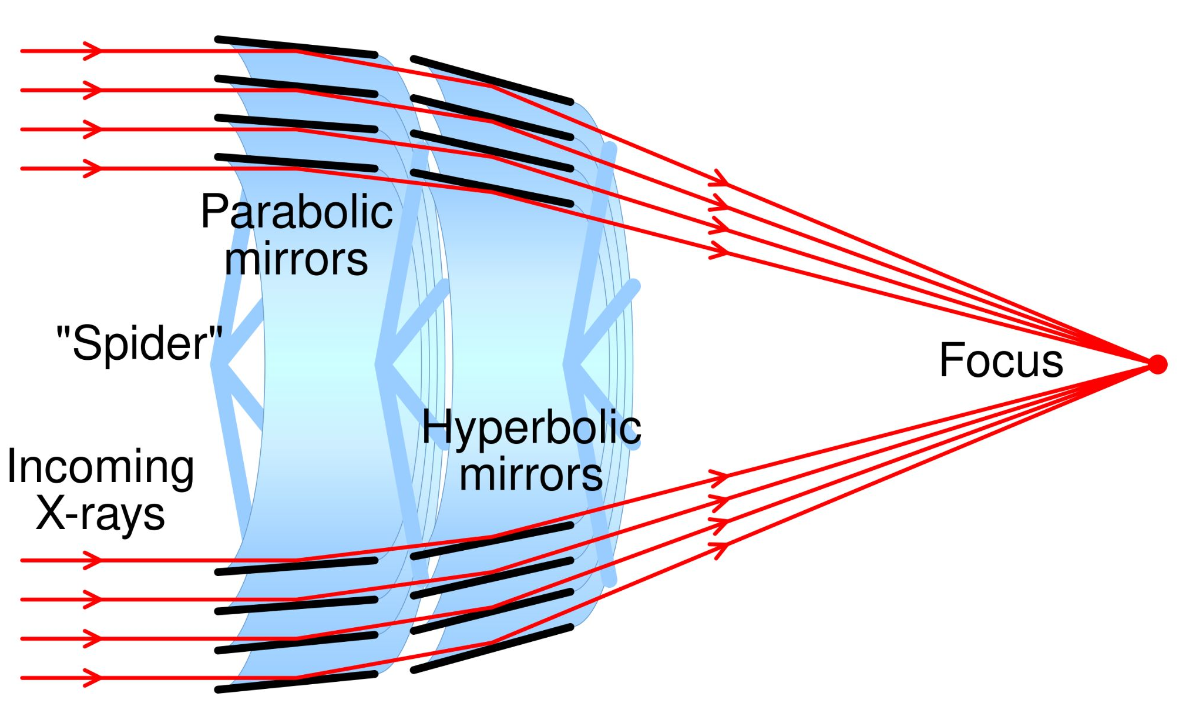
\includegraphics[width=\textwidth]{assets/x-rays.png}
\end{minipage}

The trade-offs are that X-ray mirrors are quite massive, focal lengths are long, and the resulting fields of view are small. Off-axis aberrations are controllable but remain a significant challenge.

\begin{observationblock}[Image quality in X-ray telescopes]
The angular resolution of X-ray telescopes is \textbf{not} limited by diffraction: given the extremely short wavelengths involved, the diffraction limit would be vanishingly small. Instead, the delivered resolution is governed by imperfections in the crystalline structure of the metallic mirror surfaces and by the alignment precision of the nested mirror shells, both of which become more critical at larger off-axis angles.
\end{observationblock}

The efficiency of grazing-incidence reflection depends strongly on photon energy: the critical angle for total reflection decreases with increasing radiation energy. Higher-energy photons scatter only at the most extreme grazing angles, which limits the effective energy range of Wolter-type telescopes to approximately 0.1--15\,keV (the \textbf{soft X-ray} regime).

\begin{table}[ht]
    \centering
    \caption{Angular resolution (PSF width) as a function of off-axis angle for X-ray observatories.}
    \renewcommand{\arraystretch}{1.15}
    \begin{tabular}{lcccccc}
        \toprule
        \textbf{Observatory} & \textbf{Energy [keV]} & \textbf{0$'$} & \textbf{5$'$} & \textbf{10$'$} & \textbf{20$'$} \\
        \midrule
        ROSAT    & 1     & $3''$   & $3''$   & $7''$   & $26''$ \\
        XMM      & $<2.5$ & $20''$  & --      & --      & --     \\
        Chandra  & --    & $<1''$  & $2''$   & $5''$   & $20''$ \\
        \bottomrule
    \end{tabular}
\end{table}


\subsection{X-ray Detectors} \label{subsec:xray_detectors}

Most current X-ray telescopes (including XMM-Newton and Chandra) employ CCD detectors, similar in principle to those used in optical astronomy but operated in a fundamentally different regime. Because each X-ray photon carries sufficient energy to liberate many electron-hole pairs in silicon (rather than the single electron produced by an optical photon), the CCD functions as a \textbf{photon-counting spectrometer}: both the position and the energy of each incoming X-ray are measured at readout.

The detection process proceeds as follows. Each incoming X-ray photon produces a cloud of many electrons, with the total charge proportional to the photon energy. This charge event is typically spread over several neighbouring pixels. The mean position of the charge distribution yields the arrival position of the photon on the detector, while the total integrated charge gives the photon energy. Detectors must be read out rapidly; if two events overlap in pixel space (a condition known as \textbf{pile-up}), they cannot be disentangled, leading to spectral and positional distortions.

% TODO: add image of XMM-Newton MOS camera CCDs


\subsection{X-ray Missions} \label{subsec:xray_missions}

\subsubsection{ROSAT}

The Röntgen Satellite (ROSAT) conducted the first all-sky X-ray survey, cataloguing 18\,811 sources with a limiting PSPC count rate of 0.05\,cts/s in the 0.1--2.4\,keV energy band. The ROSAT sky map in the 0.5--0.9\,keV (3/4\,keV) band reveals X-ray emission from million-degree plasmas: stellar coronae, supernova remnants, superbubbles, and the hot plasma of the Galactic nucleus. Superimposed on these Galactic structures is a weak, nearly isotropic extragalactic background produced by the superposition of unresolved active galaxies and galaxy clusters.

% TODO: add ROSAT sky map figure

\subsubsection{eROSITA}

The extended ROentgen Survey with an Imaging Telescope Array (eROSITA) represents a major advance over ROSAT. The instrument consists of seven independent Wolter-type telescope modules, each equipped with approximately 30 concentric nested grazing-incidence mirrors, a $1°$ diameter field of view, a collecting area comparable to that of ROSAT, and an angular resolution of ${\sim}\,30''$. Each module is coupled to a position- and energy-sensitive CCD detector.

eROSITA operates at the Sun-Earth L2 Lagrange point. The satellite rotates around the Sun-spacecraft axis, scanning a great circle on the sky approximately $90°$ from the Sun. As the Earth orbits the Sun, this scan sweeps across the entire celestial sphere, completing one full-sky survey every six months.

Launched by Roscosmos on 13 July 2019, eROSITA began collecting scientific data in October 2019. The first all-sky survey was completed on 11 June 2020, cataloguing 1.1 million sources. The source population is dominated by active galactic nuclei (${\sim}\,77\%$), followed by magnetically active stars with hot coronae (${\sim}\,20\%$) and galaxy clusters (${\sim}\,2\%$), along with X-ray binaries, supernova remnants, extended star-forming regions, and transients such as gamma-ray bursts. Data collection was suspended on 26 February 2022 following the breakdown of institutional cooperation between Germany and Russia.

% TODO: add eROSITA images (interacting clusters and/or all-sky map)

\subsubsection{Astro-H (HITOMI) and XRISM}

The Astro-H satellite (HITOMI), a JAXA X-ray astronomy mission, was designed to achieve unprecedented spectral resolution in the X-ray band. Its instrument suite comprised two soft X-ray telescopes (0.4--12\,keV) with a micro-calorimeter spectrometer achieving a remarkable 5\,eV spectral resolution (compared to the 100--150\,eV resolution of conventional CCD spectrometers), two hard X-ray telescopes (5--80\,keV), and two soft gamma-ray detectors (60--600\,keV). Despite its scientific promise, the mission lasted only approximately 37.5 days (of a planned three-year lifetime) before a spacecraft attitude control failure led to its loss in March 2016.

The \textbf{X-Ray Imaging and Spectroscopy Mission} (XRISM), launched in September 2023, is the direct successor to HITOMI. It carries a micro-calorimeter spectrometer providing the same exceptional spectral resolution, opening a new window onto the dynamics, temperature structure, and chemical composition of hot astrophysical plasmas in galaxy clusters, supernova remnants, and accretion flows around compact objects.


\subsection{Gamma-ray Observatories} \label{subsec:gamma_observatories}

\subsubsection{Fermi Gamma-ray Space Telescope}

The Fermi Gamma-ray Space Telescope (NASA, launched 2008) carries two complementary instruments. The \textbf{Large Area Telescope} (LAT) is an imaging gamma-ray detector sensitive from 20\,MeV to 300\,GeV, with a field of view spanning approximately 20\% of the sky. Its angular resolution improves with energy, from ${\sim}\,3.5°$ at 100\,MeV to better than $0.15°$ above 10\,GeV. The \textbf{Gamma-ray Burst Monitor} (GBM) consists of 14 scintillation detectors covering 8\,keV to 30\,MeV, capable of detecting gamma-ray bursts across the entire sky not occulted by the Earth.

Fermi's key scientific objectives include: understanding particle acceleration mechanisms in AGN, pulsars, and supernova remnants; resolving unidentified gamma-ray sources and characterising the diffuse emission; determining the high-energy properties of gamma-ray bursts and transients; and probing dark matter through searches for anomalous gamma-ray emission (for example, from the Galactic centre).

% TODO: add Fermi LAT full-sky map figure

\subsubsection{Cherenkov Telescope Array Observatory (CTAO)}

The CTAO is the next generation of ground-based gamma-ray observatory, covering the energy range from ${\sim}\,10$\,GeV to ${\sim}\,300$\,TeV with an angular resolution of $\leq 0.05°$ and an energy resolution of ${\sim}\,10\%$. Unlike satellite instruments, the CTAO detects gamma rays indirectly through the \textbf{Cherenkov radiation} produced by electromagnetic air showers in the Earth's atmosphere.

When a primary gamma-ray photon interacts in the upper atmosphere, it initiates an electromagnetic cascade (air shower) of relativistic charged particles. These particles travel faster than the local phase velocity of light in air and emit \bfit{Cherenkov light}: coherent optical and near-UV radiation ($\lambda \sim 300$--$600$\,nm) in the form of a nanosecond-duration optical flash. The resulting light pool on the ground spans approximately 120--250\,m in diameter and is imaged by arrays of telescopes equipped with fast photodetectors.

By combining stereoscopic images from multiple telescopes, the CTAO can reconstruct the shower geometry, achieve its target angular and energy resolution, and effectively suppress the hadronic cosmic-ray background that dominates at these energies.

The CTAO will consist of two complementary arrays:

\begin{itemize}
    \item \textbf{Southern site} (Atacama Desert, Chile): 4 Large-Sized Telescopes (LST) + 25 Medium-Sized Telescopes (MST) + 70 Small-Sized Telescopes (SST), providing full coverage from 20\,GeV to 300\,TeV.
    \item \textbf{Northern site} (La Palma, Canary Islands): 4 LST + 15 MST, covering 20\,GeV to 20\,TeV.
\end{itemize}

\begin{figure}[H]
    \centering
    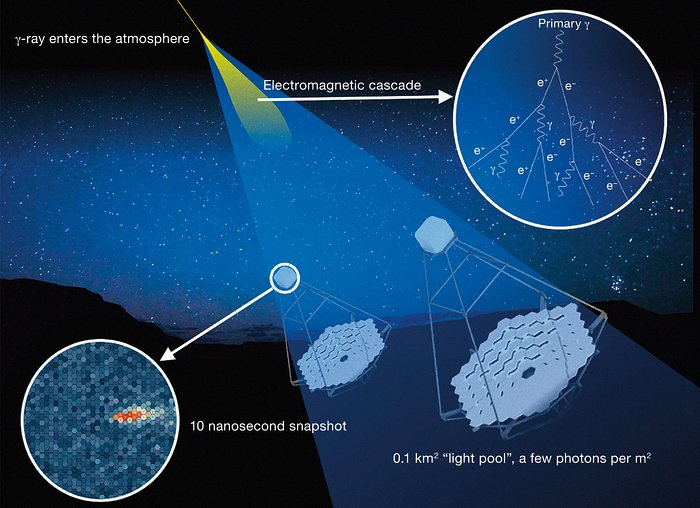
\includegraphics[width=0.5\textwidth]{assets/ctao.jpg}
    \caption{CTAO won't be detecting gamma rays directly. It will pick up Cherenkov light, the blue flash of light resulting from gamma rays interacting with the Earth's atmosphere.}
    \label{fig:ctao}
\end{figure}

\subsubsection{HERMES}

\todo{Complete HERMES mission description.}